% \documentclass[12pt,a4paper]{report}
\documentclass[11pt,a4paper]{postdoc_temp}
% \documentclass[a4paper,12pt,twoside]{postdoc_temp}

% Include necessary packages
\usepackage[utf8]{inputenc}
\usepackage{graphicx}
\usepackage{amsmath}
\usepackage{amssymb}
\usepackage{geometry}
\usepackage[colorlinks]{hyperref}
\geometry{a4paper, margin=1in}

% Include packages for todo notes
\usepackage{lineno} % in preamble
\usepackage[table]{xcolor}
\usepackage[colorinlistoftodos]{todonotes}
% \usepackage[disable]{todonotes}  % To disable todo notes, uncomment this line

% Include custom CMS definitions
\usepackage{ptdr-definitions}
% \usepackage{topcapt} % Deprecated, use caption instead
\usepackage[justification=centering]{caption}

% For table and subfigures
\usepackage{tabularx}
% Use one subfigure package only
\usepackage{subfig}

%%%%%%%%%%%%%%%%%%%%%%%%%%%%%%%%%%%%%%%%
% Style of chapter headings: START
%%%%%%%%%%%%%%%%%%%%%%%%%%%%%%%%%%%%%%%%
\usepackage{titlesec}
\makeatletter
\titleformat{\chapter}[frame]{\large}{\filright\enspace \@chapapp~\thechapter\enspace}{10pt}{\LARGE\bfseries\filcenter}
\titlespacing*{\chapter}{0pt}{-10pt}{50pt}
\makeatother

\fancypagestyle{biblio}{
  \renewcommand{\headrulewidth}{0.5pt}
  \setlength{\headheight}{14.5pt}
  \if@openright\cleardoublepage\else\clearpage\fi
  \fancyhead[el,or]{\thepage}
  \fancyhead[er,ol]{Bibliography}}

\fancypagestyle{ending}{
  \renewcommand{\headrulewidth}{0.5pt}
  \setlength{\headheight}{14.5pt}
  \if@openright\cleardoublepage\else\clearpage\fi
  \fancyhead[el,or]{\thepage}
  \fancyhead[er,ol]{\chapterhdrname}}
%%%%%%%%%%%%%%%%%%%%%%%%%%%%%%%%%%%%%%%%
% Style of chapter headings: END
%%%%%%%%%%%%%%%%%%%%%%%%%%%%%%%%%%%%%%%%

% Title and Author
\author{Ram Krishna Sharma}
\title{New physics searches in the Higgs boson sector at the CMS experiment}
\instZH{\zhs{中国科学院高能物理研究所}} %Institute of Theoretical Physics
\supervZH{Prof. Mingshui Chen \zhs{陈明水}}
\dateZH{\zhs{\number\year~年 \number\month~月}} % Current date year - month
\datese{\zhs{2019 年 12 月 -- 2022 年 06 月}} % Starting date (yyyy/mm) and ending date
\psectZH{\zhs{物理学}} % Primary Scientific Sector
\ssectZH{\zhs{粒子物理与原子核物理}} % Secondary scientific sector
\nclass{}
\nsecret{}
\udc{}
\nschem{}

% Include additional files
\includeonly{
    abstract,
    chapters/introduction,
    chapters/diHiggsSearcehs,
    chapters/highMassSearches,
    % chapters/differentialFiducialXS_H4l,
    % chapters/EFTStudies,
    chapters/aTGC,
    % chapters/massMeasurement,
    % chapters/VH,
    % chapters/egamma,
    % chapters/hgcal,
    % chapters/results,
    % chapters/conclusion,
    appendix/appendix,
    appendix/ModifiedPhotonID,
}

\begin{document}
% Uncomment for line numbers
% \linenumbers
% Uncomment for todo notes list
% \listoftodos

% Title Page
\maketitle
% Replace preambulo
\chapter*{Preface}

% Abstract
\chapter*{Abstract}
\addcontentsline{toc}{chapter}{Abstract}

% \noindent \lipsum[1-3].
% This report summarises the work done by Ram Krishna Sharma in the CMS group of the Institute of High Energy Physics,
% with Prof. Mingshui Chen, from September 2022 to December 2024.
% The main focus was on the double Higgs non-resonant production with fully Hadronic final state
% of WW$\gamma \gamma$, Higgs to 4 lepton differentical and fiducial cross-section measurement
% and vector boson scattering measurement with semi-leptonic WW final state.
% Other secondary project includes the studies with the resonant production of Higgs boson
% (performed in 2020 with 2017 data, again started with full run-2 data), CPPF, EGamma HLT studies.


The Higgs boson, a cornerstone of the Standard Model (SM), offers unique opportunities to probe the fundamental
structure of particle physics.
This thesis presents a comprehensive study of Higgs boson properties, searches for physics beyond the
Standard Model (BSM), and contributions to detector development and operation using data collected by
the CMS experiment at the CERN Large Hadron Collider (LHC).

A significant portion of this work focuses on the search for resonant Higgs boson pair production
(\(X \to HH \to WW\gamma\gamma\)), which provides insights into the Higgs self-coupling and potential
extensions of the SM.
Additionally, high-mass scalar searches (\(X \to ZZ\)) are performed to explore new resonances
predicted by BSM models.
Precision studies are conducted in the \(H \to 4\ell\) channel to measure differential and fiducial cross sections,
offering stringent tests of SM predictions.

To probe anomalous interactions, effective field theory (EFT) parameterizations and measurements of
anomalous triple gauge couplings (aTGC) are utilized.
This thesis also includes the measurement of the Higgs boson mass in the \(H \to \gamma\gamma\) channel,
providing one of the most precise determinations of this fundamental parameter.
Studies of associated Higgs production (\(VH\)) further test the Higgs boson's interactions with vector bosons.

Beyond physics analyses, contributions to the CMS detector include developments in electron and photon
reconstruction algorithms, studies of the High-Granularity Calorimeter (HGCAL) for the High-Luminosity LHC
upgrade, and participation in detector operations.

The results and conclusions presented in this thesis provide valuable insights into the properties of
the Higgs boson and offer constraints on new physics scenarios.
These contributions advance our understanding of the SM and pave the way for future discoveries at the LHC.

\vspace*{2em}

\noindent \textbf{Keywords:} {CMS experiment, VBS, HH, differential, fiducial measurement, CPPF}


% Table of Contents
\tableofcontents
\listoffigures
\listoftables

\cuerpo
\setlength{\parskip}{0.75em}

% Chapters
\include{chapters/introduction}
\chapter{Search for Resonant Di-Higgs }
\label{ch:diHiggs_search}

% \chapter{Search for Resonant Di-Higgs Production in the \texorpdfstring{\(X \to HH \to WW\gamma\gamma\)}{X->HH->WWgg} Channel}

\section{Introduction and Motivation}
The study of Higgs boson pair production provides a unique opportunity to probe the Higgs self-coupling and to search for physics
beyond the Standard Model (BSM). In the SM, Higgs boson pairs are dominantly produced via gluon-gluon fusion (ggF) through triangle
and box diagrams, as shown in Fig.~\ref{SMLO_ggHH_production}, that exhibit destructive interference.
The predicted cross section for non-resonant di-Higgs production is small, \(0.01449 \pm 0.000019\)~pb,
making this process challenging to observe.
\begin{figure}[!htbp]
    \begin{center}
        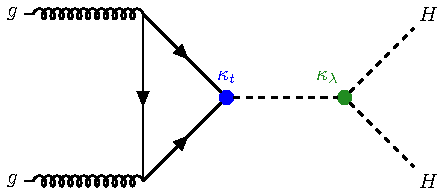
\includegraphics[width=0.45\textwidth]{figures/diHiggsSearches/fey_HH_Triangle.pdf} %
        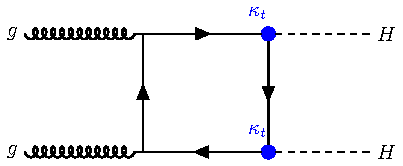
\includegraphics[width=0.45\textwidth]{figures/diHiggsSearches/fey_HH_Box.pdf}
    \end{center}
    \caption{Feynman diagrams for leading-order Higgs boson pair production via gluon fusion}
    \label{SMLO_ggHH_production}
\end{figure}
\begin{figure}[!htbp]
    \begin{center}
        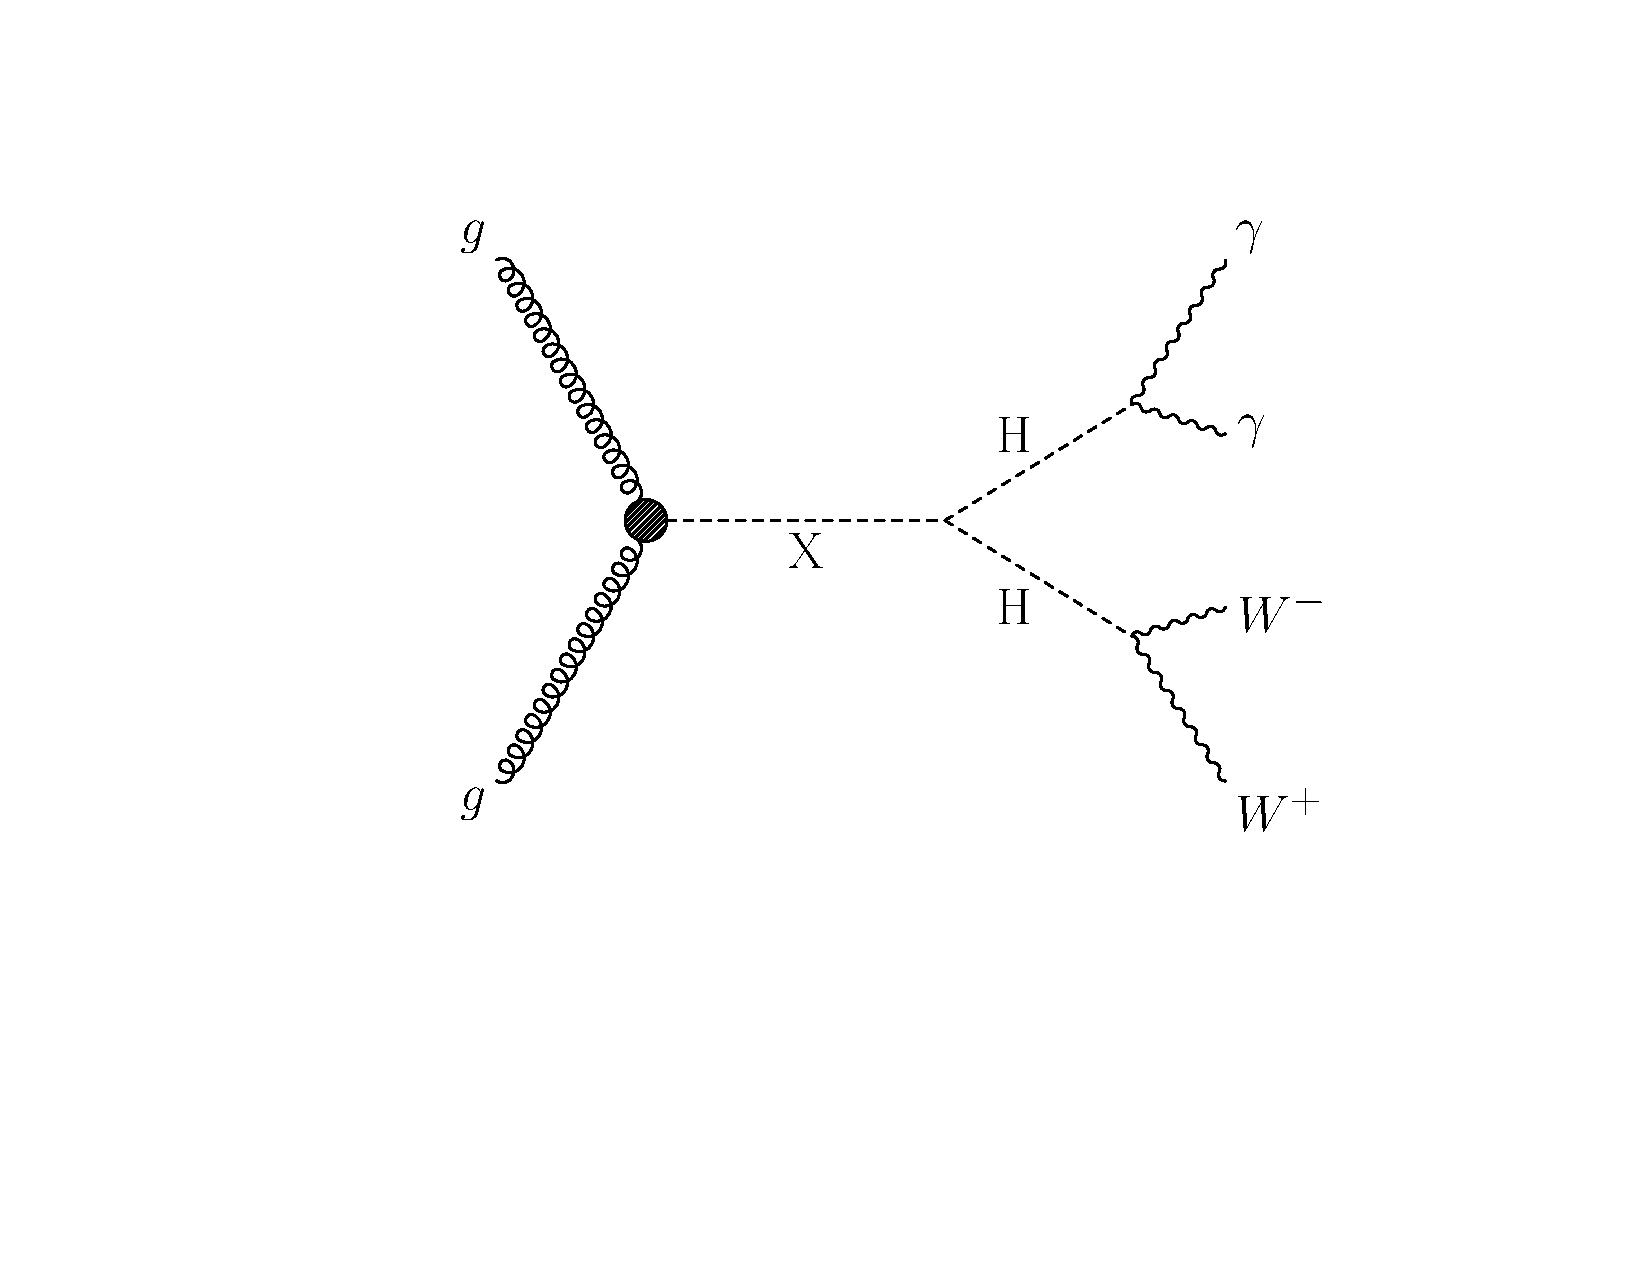
\includegraphics[width=0.45\textwidth]{figures/diHiggsSearches/fey_XHH_HHWWgg.pdf}
    \end{center}
    \caption{Feynman diagram for resonant di-Higgs production in the \HH channel}
    \label{XHHFeynmanDiagram}
\end{figure}


Extensions of the SM, such as the Next-to-Minimal Supersymmetric Standard Model (NMSSM), Randall-Sundrum models, or the two-Higgs
doublet model (2HDM), predict resonant di-Higgs production. In these scenarios, a heavy resonance \(X\) decays into two Higgs
bosons, which subsequently decay into \(WW\) and \(\gamma\gamma\), as shown in Fig.~\ref{XHHFeynmanDiagram}. This analysis specifically focuses on \(X \to HH \to
WW\gamma\gamma\), leveraging the clean diphoton final state to enhance sensitivity while covering all possible jet topologies.


\section{Analysis Overview}
The analysis is performed using the full Run-2 Ultra-Legacy dataset, corresponding to an integrated luminosity of 138~fb\(^{-1}\) at
\(\sqrt{s} = 13\)~TeV. The following decay channels are explored:
\begin{itemize}
    \item \textbf{Semi-leptonic (\(l\nu qq\gamma\gamma\)):} One \(W\) boson decays leptonically (\(W \to l\nu\)), and the other
    decays hadronically (\(W \to qq\)).
    \item \textbf{Fully hadronic (\(4q\gamma\gamma\)):} Both \(W\) bosons decay hadronically (\(W \to qq\)).
\end{itemize}

\section{Unique Features of the Analysis}
This analysis incorporates several innovative aspects, as detailed below:

\begin{itemize}
    \item \textbf{Comprehensive Topology Coverage:}
    For the first time, all jet topologies are tagged within a single analysis. These include boosted, semi-boosted, resolved, and scenarios where leptons are reconstructed inside jets.

    \item \textbf{Signal Definition:}
    The signal is defined as the sum of three di-Higgs decay possibilities:
    \[
    HH \to WW\gamma\gamma + ZZ\gamma\gamma + bb\gamma\gamma.
    \]
    Since the hadronic decay topologies are similar for all three channels, it is challenging to reduce contamination from the \(ZZ\gamma\gamma\) and \(bb\gamma\gamma\) channels in our primary signal of interest, \(WW\gamma\gamma\). The signal definition is further refined with the following considerations:
    \begin{itemize}
        \item The analysis is optimized for the \(HH \to WW\gamma\gamma\) channel.
        \item For \(HH \to WW\gamma\gamma\), two decay modes of the \(W\)-bosons are considered: fully hadronic and semi-leptonic. The analysis optimization is performed based on these two final states.
        \item For \(HH \to ZZ\gamma\gamma\), due to the low branching fraction and negligible semi-leptonic contribution, the semi-leptonic decay mode is excluded from the analysis.
        \item The \(bb\gamma\gamma\) channel is included after applying a b-jet veto. This serves multiple purposes:
        \begin{enumerate}
            \item It reduces the contribution from the \(bb\gamma\gamma\) channel, ensuring that the limit is primarily driven by the \(WW\gamma\gamma\) channel rather than \(bb\gamma\gamma\).
            \item It makes the analysis orthogonal to the \(HH \to bb\gamma\gamma\) analysis.
            \item Events rejected by the \(HH \to bb\gamma\gamma\) analysis are exploited, thereby utilizing additional information from the same dataset.
            \item The b-jet veto also rejects events from \(HH \to ZZ\gamma\gamma\) where the \(Z\)-bosons decay into b-quarks.
        \end{enumerate}
    \end{itemize}

    \item \textbf{Mass Ranges:}
    The resonance \(X\) is studied over a mass range of 250~GeV to 3000~GeV.

    \item \textbf{Leptons Inside Jets:}
    Events where leptons are reconstructed within jets are included, thereby enhancing sensitivity to specific Beyond Standard Model (BSM) scenarios.
\end{itemize}

\section{Event Selection}


The event selection optimizes sensitivity to semi-leptonic and fully hadronic channels, with the following criteria:

\subsection*{Photon Selection}
\begin{itemize}
    \item A boosted decision tree (BDT) classifier is trained to separate photons from jets~\cite{Sirunyan:2018ouh}.
            The output of this BDT is referred to as the photon ID score
            \footnote{For the boosted regime, where the two photons are close by, the photon ID score was modified to
            account for reduced selection efficiency.
            This modified score is referred to as the ``modified photon ID," detailed in
            Appendix~\ref{appendix:ModifiedPhotonID}}.
    \item Leading photon \(p_T > 35\)~GeV and subleading photon \(p_T > 25\)~GeV.
    \item Photon transverse momentum fractions: \(p_T/m_{\gamma\gamma} > 0.33\) (leading) and \(> 0.25\) (subleading).
    \item Diphoton invariant mass requirement: \(100 < m_{\gamma\gamma} < 180\)~GeV.
\end{itemize}


\subsection*{Lepton Selection}
\begin{itemize}
    \item \todo[inline]{Missing the ID for isolated as well as non-isolated leptons}
    \item Isolated leptons: \(p_T > 10\)~GeV, \(|\eta| < 2.4\), with \(\Delta R(l,\gamma) > 0.4\)
    \item Non-isolated leptons: \(\Delta R(l, \text{FatJet}) < 0.8\), with relaxed isolation criteria.
    \item \(Z\)-veto: \(|m_{l\gamma} - 91.2| > 5\)~GeV to suppress \(Z\)-boson contamination.
\end{itemize}

\subsection*{Jet Selection}
\begin{itemize}
    \item AK4 jets: \(p_T > 30\)~GeV, \(|\eta| < 2.4\), passing tight jet ID \todo[inline]{Define ID}.
    \item AK8 jets: \(p_T > 200\)~GeV, \(|\eta| < 2.4\), with jet mass consistent with \(W\)- or Higgs-like jets.
    \item Boosted Higgs tagging uses ParticleNet \todo[inline]{define particleNet in the footnote} with a score threshold of 0.2.
\end{itemize}

\subsection*{Event Topologies}
Four jet categories are defined:
\begin{itemize}
    \item \textbf{1-jet:} A single AK8 jet tagged as a Higgs jet.
    \item \textbf{2-jet:} Two AK8 jets, one tagged as a Higgs jet and the other as a \(W\)-jet.
    \item \textbf{3-jet:} One AK8 jet combined with two AK4 jets.
    \item \textbf{4-jet:} Fully resolved topology with four AK4 jets.
\end{itemize}


\section{Data-Driven Background Estimation}
Accurate estimation of backgrounds is crucial for isolating the signal in the \(X \to HH \to WW\gamma\gamma\) analysis.
The dominant backgrounds include non-resonant diphoton production, single Higgs processes, and multijet events
where fake photons mimic the signal.
A data-driven strategy is employed to estimate fake photon backgrounds, inspired by CMS analysis HIG-19-013.

\subsection{Motivation}
The low statistics of QCD Monte Carlo (MC) samples result in poor modeling of important input features to multivariate analyses. To
ensure agreement between data and MC and unbiased training of machine learning models, a data-driven approach is adopted. The method
uses events from the photon ID MVA sideband to model fake photon contributions.

\subsection{Methodology}
The following steps outline the data-driven background estimation strategy:

\begin{enumerate}
    \item \textbf{Photon ID Sideband Selection:}
    Events that fail the preselection cut on the photon ID MVA are used to model fake photons. The sideband regions are chosen as:
    \begin{itemize}
        \item Resolved category: Minimum photon ID MVA in the range \([-0.9, -0.7]\),
        \item Boosted category: Minimum photon ID MVA in the range \([-0.95, -0.9]\).
    \end{itemize}

    \item \textbf{PDF Generation for Fake Photons:}
    A probability density function (PDF) for the photon ID MVA distribution of fake photons is obtained from MC samples (e.g.,
    \(\gamma + \text{jets}\)). The sideband events are reweighted to match the fake photon PDF in the signal region.

    \item \textbf{Reweighting and Normalization:}
    Events in the photon ID sideband are assigned per-event weights to reshape the maximum photon ID MVA distribution. The weight
     \(w\) is defined as:
    \begin{equation}
        w = \frac{\int_{\text{minID}}^{\text{maxID}} \text{fakePDF}(x) \, dx}
                 {\int_{\text{sidebandMinID}}^{\text{sidebandMaxID}} \text{fakePDF}(x) \, dx}.
    \end{equation}
    Different weight functions are applied for resolved and boosted categories.

    \item \textbf{Validation:}
    The reweighted MC is normalized to data to ensure consistency. Comparisons before and after applying the data-driven method demonstrate improved agreement in key variables, such as \(m_{\gamma\gamma}\).
\end{enumerate}

\subsection{Challenges and Solutions}
The data-driven method is validated for both fully hadronic (FH) and semi-leptonic (SL) channels. However, specific challenges arise:
\begin{itemize}
    \item \textbf{Muon Channel in SL Events:}
    While the method improves data-MC agreement in the electron channel, it worsens agreement in the muon channel. Possible solutions include:
    \begin{itemize}
        \item Use the data-driven approach for the electron channel only.
        \item Perform separate reweighting for the electron and muon channels.
    \end{itemize}
    Currently, a combined reweighting technique is applied to correct control plots, ensuring consistent results without relying
    heavily on MC samples.

    \item \textbf{Photon ID Sidebands:}
    Assumptions underlying the sideband method include:
    \begin{enumerate}
        \item Other variables used in the analysis are minimally correlated with the photon ID MVA.
        \item The low photon ID sideband is dominated by fake photons (e.g., from QCD and \(\gamma + \text{jets}\)).
        \item Photons in the low ID sideband are always fake.
    \end{enumerate}
\end{itemize}

\subsection{Implementation in Different Channels}
The method is applied to both fully hadronic and semi-leptonic channels:
\begin{itemize}
    \item \textbf{Fully Hadronic Channel:}
    Dominated by QCD backgrounds, where the photon ID MVA sideband reliably models fake photon contributions.
    \item \textbf{Semi-Leptonic Channel:}
    Includes fake photon contributions from \(W\gamma\gamma\) and \(t\bar{t}\) processes, with non-isolated leptons contributing to
    the final background estimation.
\end{itemize}

\subsection{Impact of the Data-Driven Method}
The results of the data-driven background estimation are as follows:
\begin{itemize}
    \item Significant improvement in the modeling of photon-related variables in both resolved and boosted categories.
    \item Enhanced agreement between data and MC distributions in control regions, as shown in Figure~\ref{fig:control_plots}.
    \item Improved sensitivity to the \(X \to HH \to WW\gamma\gamma\) signal, particularly in high-mass regions.
\end{itemize}

The control plots for the resolved and boosted regions before and after applying the data-driven method demonstrate the
effectiveness of this strategy. Future improvements will address challenges in the muon channel and refine the photon ID sideband
methodology.

\section{Multivariate Analysis Using Parameterized Neural Network (pNN)}

To maximize the sensitivity of the search for resonant \(X \to HH \to WW\gamma\gamma\), a multivariate analysis (MVA) is performed
using a Parameterized Neural Network (pNN). The pNN method allows for simultaneous training across multiple signal hypotheses,
parameterized by the mass of the heavy resonance \(m_X\). This approach ensures a more robust discrimination between signal and
background across a wide range of masses, from 250~GeV to 3000~GeV.

\subsection{Overview of pNN Methodology}
The pNN method is implemented as a deep feed-forward neural network. The network inputs include kinematic and topological features of the events, while the resonance mass \(m_X\) is used as a parameter to generalize the signal hypothesis. The key features of the pNN method are:
\begin{itemize}
    \item \textbf{Parameterized Mass Input:} The network is trained with the resonance mass \(m_X\) as an input variable, enabling simultaneous training for multiple signal mass points.
    \item \textbf{Dropout Layer:} Introduced to prevent overtraining and enhance generalization.
    \item \textbf{Optimizer:} The Adam optimizer is used for training with stochastic gradient descent.
    \item \textbf{GPU-Based Training:} Training is accelerated using GPUs for efficient processing of large datasets.
\end{itemize}

\subsection{Training Strategy}
Separate pNNs are trained for the **boosted** and **resolved** topologies due to the distinct event kinematics in these categories:
\begin{itemize}
    \item \textbf{Boosted Category:} Events where \(W\)-bosons' decay products are merged into single AK8 jets.
    \item \textbf{Resolved Category:} Events where \(W\)-bosons' decay products are reconstructed as individual AK4 jets.
\end{itemize}

The input features for the pNN are selected based on their ability to discriminate signal from background. These features include photon, jet, and missing transverse energy (\(E_T^{\text{miss}}\)) observables.

\subsection{Input Features}
The key input variables used for training the pNN are listed in Tables~\ref{tab:pnn_boosted_inputs} and \ref{tab:pnn_resolved_inputs}.

\begin{table}[h!]
    \centering
    \caption{Input variables for the pNN in the boosted category.}
    \label{tab:pnn_boosted_inputs}
    \begin{tabular}{ll}
        \hline
        \textbf{Feature} & \textbf{Description} \\
        \hline
        Diphoton \(p_T/m_{\gamma\gamma}\) & Transverse momentum of diphoton system normalized to \(m_{\gamma\gamma}\) \\
        Diphoton \(dR\) & Angular separation between leading and subleading photons \\
        Leading Photon \(p_T/m_{\gamma\gamma}\) & Leading photon \(p_T\) normalized to \(m_{\gamma\gamma}\) \\
        Subleading Photon \(p_T/m_{\gamma\gamma}\) & Subleading photon \(p_T\) normalized to \(m_{\gamma\gamma}\) \\
        FatJet \(p_T\), \(m\), \(\eta\), \(\phi\) & Transverse momentum, mass, pseudorapidity, and azimuthal angle of leading AK8 jets \\
        \(E_T^{\text{miss}}\) & Missing transverse energy \\
        FatJet-diphoton \(dR\) & Angular separation between leading fatjet and diphoton system \\
        \hline
    \end{tabular}
\end{table}

\begin{table}[h!]
    \centering
    \caption{Input variables for the pNN in the resolved category.}
    \label{tab:pnn_resolved_inputs}
    \begin{tabular}{ll}
        \hline
        \textbf{Feature} & \textbf{Description} \\
        \hline
        Diphoton \(p_T/m_{\gamma\gamma}\) & Transverse momentum of diphoton system normalized to \(m_{\gamma\gamma}\) \\
        Diphoton \(dR\) & Angular separation between leading and subleading photons \\
        Leading Jet \(p_T\), \(m\), \(\eta\), \(\phi\) & Kinematic properties of leading AK4 jets \\
        Subleading Jet \(p_T\), \(m\), \(\eta\), \(\phi\) & Kinematic properties of subleading AK4 jets \\
        Diphoton-jet \(dR\) & Angular separation between diphoton system and jets \\
        \(E_T^{\text{miss}}\) & Missing transverse energy \\
        B-jet Scores & Highest and second-highest b-tagging scores for AK4 jets \\
        \hline
    \end{tabular}
\end{table}

\subsection{Performance and Validation}
The performance of the pNN is validated using standard metrics such as the area under the curve (AUC) and signal-to-background ratio improvements. The following observations are noted:
\begin{itemize}
    \item The pNN significantly enhances discrimination between signal and background across the entire mass range.
    \item Feature importance plots indicate that the most discriminating variables are the diphoton \(p_T/m_{\gamma\gamma}\), \(dR\) between photons, and jet kinematics.
    \item Separate training for the boosted and resolved categories optimizes sensitivity in their respective regions.
\end{itemize}

\subsection{Results of the pNN Classification}
The output of the pNN is used as the final discriminant to extract the signal in the \(m_{\gamma\gamma}\) distribution. By combining the boosted and resolved topologies, the analysis achieves a 60\% improvement in sensitivity over previous results.

\subsection{Summary of pNN Method}
The parameterized neural network approach provides a powerful method for signal extraction in the \(X \to HH \to WW\gamma\gamma\) analysis. By training across multiple mass hypotheses and incorporating advanced multivariate techniques, the pNN significantly improves the sensitivity to resonant di-Higgs production.

\section{Results}
Results are interpreted in terms of cross-section limits on \(X \to HH \to WW\gamma\gamma\). Key outcomes include:
\begin{itemize}
    \item At \(m_X = 3000\)~GeV, the observed (expected) limit is 60~fb for \(X \to HH \to WW\gamma\gamma\).
    \item The analysis shows a 60\% improvement in sensitivity compared to ATLAS at 500~GeV.
    \item Incorporating leptons inside jets enhances sensitivity, particularly in semi-leptonic topologies.
\end{itemize}

\section{Systematic Uncertainties}
Major systematic uncertainties include:
\begin{itemize}
    \item QCD scale variations for high-mass resonances.
    \item Photon energy resolution and identification efficiency.
    \item Jet energy scale and resolution.
\end{itemize}

The impact of these uncertainties is quantified and incorporated into the statistical interpretation.

\section{Signal and Background Modelling}
\label{sec:signal_background_modelling}

The extraction of the \(X \to HH \to WW\gamma\gamma\) signal is performed using the same methodology as the Higgs boson analysis in the \(H \to \gamma\gamma\) channel~\cite{CMS:2020xrn}. This involves precise modelling of the signal shape using simulated samples and the background shape using data-driven techniques.

\subsection{Signal Modelling}
The signal shape is parameterized based on Monte Carlo (MC) simulations, with the diphoton invariant mass \(m_{\gamma\gamma}\) as the primary observable.

\begin{itemize}
    \item \textbf{Signal Simulation:}
    \begin{itemize}
        \item Signal samples are generated at leading order (LO) using \textsc{MadGraph5\_aMC@NLO} for the gluon-gluon fusion process \(gg \to X\).
        \item Subsequent parton showering and hadronization are performed with \textsc{Pythia8}, and detector effects are simulated using the CMS \textsc{Geant4}-based framework.
        \item Simulated samples are produced for resonance masses \(m_X\) ranging from 250~GeV to 3000~GeV.
    \end{itemize}

    \item \textbf{Signal Shape:}
    \begin{itemize}
        \item The diphoton mass distribution for the signal is modelled using a double-sided Crystal Ball (CB) function, defined as:
        \[
        f_{\text{CB}}(x) =
        \begin{cases}
            A \exp\left(-\frac{(x-\mu)^2}{2\sigma^2}\right), & \text{for } |x-\mu| \leq \alpha\sigma, \\
            B \left(\frac{n}{\alpha} - \frac{n}{\alpha - (x-\mu)/\sigma} \right)^{-n}, & \text{for } x-\mu > \alpha\sigma,
        \end{cases}
        \]
        where \(\mu\) is the mean, \(\sigma\) is the width, and \(\alpha\), \(n\) define the tail parameters.
        \item The parameters of the Crystal Ball function are extracted from fits to the MC simulation in each analysis category (boosted and resolved).
        \item The normalization of the signal is determined from the integrated luminosity and the predicted cross section for \(X \to HH \to WW\gamma\gamma\).
    \end{itemize}

    \item \textbf{Signal Categories:}
    The analysis is divided into multiple categories to maximize sensitivity:
    \begin{itemize}
        \item \textbf{Boosted:} Events where the \(W\)-boson decay products are merged into single large-radius jets.
        \item \textbf{Resolved:} Events where the \(W\)-boson decay products are reconstructed as separate small-radius jets.
        \item \textbf{Semi-leptonic and fully hadronic:} These subcategories depend on the final-state reconstruction of leptons or jets.
    \end{itemize}
\end{itemize}

\subsection{Background Modelling}
The dominant background arises from SM non-resonant diphoton production, with additional contributions from single Higgs production and fake photon processes. The background is modelled using the following approaches:

\begin{enumerate}
    \item \textbf{Non-Resonant Diphoton Background:}
    \begin{itemize}
        \item The continuum diphoton background is modelled directly from data using a smooth analytic function. This function is chosen based on its ability to fit the diphoton invariant mass sidebands while avoiding bias in the signal region.
        \item A range of functional forms, such as exponentials, power laws, or Bernstein polynomials, is tested. The optimal choice is selected using the Fisher F-test and evaluated for bias using pseudo-experiments.
        \item The background shape parameters are determined from fits to the \(m_{\gamma\gamma}\) sideband regions (\(100 < m_{\gamma\gamma} < 120\)~GeV and \(130 < m_{\gamma\gamma} < 180\)~GeV).
    \end{itemize}

    \item \textbf{Resonant Backgrounds:}
    \begin{itemize}
        \item Single Higgs production (\(ggH\), VBF, \(VH\)) with \(H \to \gamma\gamma\) is a subdominant but irreducible background. It is modelled using MC simulation normalized to the theoretical cross sections.
        \item Other rare processes such as \(t\bar{t}\gamma\gamma\), \(W\gamma\gamma\), and \(Z\gamma\gamma\) are also estimated from MC samples.
    \end{itemize}

    \item \textbf{Fake Photon Background:}
    \begin{itemize}
        \item Events where jets or electrons are misidentified as photons are estimated using a data-driven method based on the photon ID MVA sideband technique (Section~\ref{sec:data_driven_bkg}).
        \item The contribution of fake photons is validated in control regions enriched with QCD multijet events.
    \end{itemize}
\end{enumerate}

\subsection{Systematic Uncertainties}
The systematic uncertainties affecting the signal and background modelling include:
\begin{itemize}
    \item \textbf{Signal Modelling:}
    \begin{itemize}
        \item Uncertainty in the Crystal Ball function parameters.
        \item Theoretical uncertainties in the signal cross section due to renormalization and factorization scales.
    \end{itemize}
    \item \textbf{Background Modelling:}
    \begin{itemize}
        \item Uncertainties in the choice of the analytic function for the non-resonant background.
        \item Statistical uncertainties in the fits to sideband data.
    \end{itemize}
    \item \textbf{Experimental Uncertainties:}
    \begin{itemize}
        \item Photon energy scale and resolution uncertainties.
        \item Jet energy scale (JES) and jet energy resolution (JER) uncertainties.
        \item Integrated luminosity uncertainty of 1.6\%.
    \end{itemize}
\end{itemize}

\subsection{Result Extraction}
The signal extraction is performed using an unbinned maximum likelihood fit to the diphoton invariant mass spectrum \(m_{\gamma\gamma}\) in each analysis category. The signal and background components are parameterized as:
\[
f_{\text{total}}(m_{\gamma\gamma}) = N_{\text{sig}} f_{\text{sig}}(m_{\gamma\gamma}) + N_{\text{bkg}} f_{\text{bkg}}(m_{\gamma\gamma}),
\]
where \(f_{\text{sig}}\) is the signal shape modelled by the Crystal Ball function, and \(f_{\text{bkg}}\) is the smooth analytic function for the non-resonant background.

The parameters \(N_{\text{sig}}\) and \(N_{\text{bkg}}\) are extracted simultaneously through the likelihood fit, with systematic uncertainties incorporated as nuisance parameters.


\section{Signal and background modelling} \label{sec:AnalyticFitting}

In order to model the di-Higgs signal process, and single higgs resonant background processes in the signal region, 115 $< \mgg < $ 135 GeV, simulated events
in each analysis category are combined to construct $\mgg$ shapes. Because the continuum background in the signal region is expected to follow a falling
shape continuous with the data sidebands, data events in the data sidebands are fit to a falling analytic function in order to model the continuum background.

\subsection{Di-Higgs signal}
\label{sec:SignalFitting}

Signal shapes for the invariant mass distribution of the diphoton candidate are derived for all analysis categories using simulated events.

Signal models are formed by an analytic fit of a sum of 1-5 Gaussians to a binned $\mgg$ distribution, where the chosen number of Gaussians used in the fit is
determined by an F-test. This is done separately for each year (2016, 2017, 2018) and each analysis category.
The fit for the second highest DNN score region FH category is shown
in Fig.  \ref{fig:FHSignalModel} .

\missingfigure[figwidth=0.75\textwidth]{FH signal model in the second most sensitive category}
\label{fig:FHSignalModel}

% \begin{figure}[!htbp]
%   \centering
%   \includegraphics[width=0.75\textwidth,height=7cm]{Images/AnalyticFitting/Signal/smodel_HHWWggTag_FHDNN_1.pdf}
%   \caption{FH signal model in the second most sensitive category}
% \label{fig:FHSignalModel}
% \end{figure}

\subsection{Single Higgs background}

There are expected resonant background processes present in the signal region, $115 < \mgg < 135$ GeV, due to $H\rightarrow\gamma\gamma$ processes, which cannot be modeled with a data-driven
method using data sideband events. These backgrounds are modeled with MC in the same fashion as the $HH\rightarrow WW\gamma\gamma$ signals as described in Sec. \ref{sec:SignalFitting}. The single higgs
processes considered as resonant backgrounds are the gluon-gluon fusion, vector boson fusion, associated production with a vector boson, and associated production with a top quark pair (ttH), where the Higgs boson decays
into two photons. A separate fit is made for each analysis category and production mode. For cases in which there is a very small number of MC statistics, the diphoton shape from
the di-Higgs signal model in the same analysis category is taken and scaled to the single higgs yield in this category, and used to model the single higgs shape in this category.

\subsection{Continuum background}
\label{sec:AnalyticFitting_Background}

A data-driven background model is produced for each category using the data sidebands in the regions $100 < \mgg < 115$ GeV and $135 < \mgg < 180$ GeV.
The aim of this is to model the continuum background.
After the event selections and categorizations described in Sec. \ref{sec:event_selection} are applied, analytic functions are fit to the resulting $\mgg$ distributions in the data sidebands for each category.
These are later combined with their corresponding signal models in order to extract final results.
As with the signal fitting, an F-Test is performed first in order to obtain initial best-fit estimates for backgrounds functions to the data-sidebands, and to determine which functions will be considered.
Bernstein, laurent, exponential, and powerlaw function families are considered as
candidates to fit the data, and F-Tests are performed for each of these. The three data taking years are merged together before the F-test and function fitting is performed.
After determining which functions pass the F-Test, a best fit function is chosen with the envelope method by treating the choice of function as a discrete nuisance parameter.
An uncertainty is then assigned to the chosen fit function based on a combination of the likelihoods of all attempted fit functions. This method is described in
Ref. \cite{Dauncey_2015}.

After obtaining signal models, continuum background models and Single-Higgs models for each final state, a signal plus background fit is performed.
The combination of all categories' signal plus background fits in the range 100 $<$ $\mgg$ $<$ 180 GeV, where each category is weighted by S over S$+$B, is shown in Figure \ref{fig:Run2SplusB}.

\missingfigure[figwidth=0.7\textwidth]{Combined limit}
\label{fig:Run2SplusB}

% \begin{figure}[!htbp]
%   \centering
%   \includegraphics[width=0.7\textwidth,height=8cm]{Images/Results/All_combined_SplusB.pdf}
%  \caption{The observed diphoton mass distribution including the signal plus background fit (red), the Single-Higgs + continuum background fit (blue) and the continuum background (black dashed line),
%  with bands covering the $\pm 1\sigma$ and $\pm 2\sigma$ uncertainties in the fitted background where all analysis categories are combined and weighted by S over S$+$B.}
%   \label{fig:Run2SplusB}
% \end{figure}

\section{Systematic uncertainties} \label{section:Systematics}
This analysis takes into account systematic uncertainties from theoretical and experimental sources. The uncertainties on the signal and on the single Higgs backgrounds are modeled as scale or shape uncertainties. The scale uncertainties affect the yield of the processes and are treated as log-normal uncertainties, while the shape uncertainties are modeled as variations of the \mgg shape of the processes, i.e. the peak position or the width. The systematic uncertainty associated with the data-driven estimate of the continuum background is accounted for via the discrete profiling method. Given the small number of expected signal events compared to the backgrounds, the effect of the systematics uncertainties on the final results is expected to be small compared to the statistical ones. In case a systematic uncertainty affects processes in different channels, it is considered fully correlated across those channels. The following sources of systematic uncertainties are considered:

\begin{enumerate}

  \item \textbf{Theoretical uncertainties on the HH cross section}: The combined uncertainty on the QCD scale and on the top mass is taken into account, considering also its dependence from the value of $\kappa_{\lambda}$. For the SM signal this uncertainty amounts to $-23/+6\% $. The combined uncertainty on the PDF modeling and on the strong coupling constant is also considered with a value of $3\% $ \cite{Grazzini:2018bsd}.

  \item \textbf{Theoretical uncertainties on the single Higgs cross sections}: Process-dependent uncertainties related to the QCD scale, the PDF modeling, and the strong coupling constant are taken into account for the ggH, ttH, VBF H, and VH processes.

  \item \textbf{Theoretical uncertainties on the Higgs boson branching ratios}: Such uncertainties are considered for both the single and the double Higgs processes. The considered uncertainties on the $H\rightarrow\gamma\gamma$, $H\rightarrow VV$, and $H\rightarrow bb$ branching ratios are approximately $2\% $, $1.5\% $, and $1.2\% $, respectively.

  \item \textbf{Integrated luminosity}: A scale uncertainty is defined according to the luminosity measurements performed by the CMS experiment ~\cite{CMS-LUM-17-003,CMS-PAS-LUM-17-004,CMS-PAS-LUM-18-002}.

  \item \textbf{Trigger}: The trigger efficiency is measured from data with a tag and probe procedure using $Z \rightarrow ee$ events. The related uncertainty is uncorrelated between the three data taking years. An additional considered source of uncertainty is related to inefficiencies of the ECAL L1 trigger at $|\eta|>2$ experienced during 2016 and 2017. This is modeled as a purely rate-changing uncertainty.

%  \item \textbf{Pile-up reweigthing}: The distribution of the simultaneous number of interactions in the Monte Carlo simulation is corrected to match the one observed in the data through an event reweight procedure. The uncertainty on the number of pile-up events is estimated by varying the proton-proton inelastic cross section, 69.2 mb, within $\pm$ 4.6\%. This is modeled as a scale uncertainty uncorrelated between the three data taking years.

  \item \textbf{Electron and muon reconstruction, identification and isolation efficiency}: These efficiencies are evaluated in data and simulation with tag-and-probe techniques using Drell-Yan events \cite{Khachatryan:2015hwa, Sirunyan:2018fpa}. Scale factors are derived and applied to the simulated events to improve the agreement of the efficiencies between simulation and data. The related uncertainty is purely rate-changing and uncorrelated between the three data taking years.

  \item \textbf{Photon identification}: The efficiency of the pre-selection on the photon identification MVA score is estimated in data and simulation with a tag-and-probe technique using Drell-Yan events. Scale factors are applied to correct for the difference between the data and the simulation. The related uncertainty is purely rate-changing  and uncorrelated between the three data taking years.

%  \item \textbf{Electron energy scale and resolution}: Corrections for the energy scale observed in the data are applied to match the simulated one, and for the energy resolution observed in the simulation to match the one observed in the data. The systematic uncertainty on the electron energy scale and resolution is taken considering the POG provided resolution error and the uncertainty on the electron $p_T$. This uncertainty is uncorrelated between the three data taking years.

  \item \textbf{Photon shower shape}: Corrections for the imperfect modeling of the photon shower shape (and isolation) variables in simulation are applied to improve the agreement with the data. The impact of this uncertainty is estimated from the difference of the photon energy scale before and after the correction. This is modeled as a shape uncertainty which is correlated between the three years of the data taking.

  \item \textbf{Photon energy scale and resolution}: Corrections for the difference of the photon energy scale and resolution between data and simulation are derived using $Z \rightarrow ee$ events, with electron-photon differences accounted for as a systematic uncertainty. This uncertainty is uncorrelated between the three years of the data taking.

% Not sure if we apply this. Check: https://github.com/atishelmanch/flashgg/blob/HHWWgg_dev/Taggers/interface/HHWWggTagProducer.h
%   \item \textbf{Di-photons vertex identification efficiency}: Scale factors are computed to account for the difference between data and simulation in number of events for which the correct vertex has been selected.

  %https://twiki.cern.ch/twiki/bin/view/CMS/JECUncertaintySources#Recommendation_for_analysis
  \item \textbf{Jet energy scale and resolution}: Corrections for the differences in the measured jet energies between data and simulation are applied \cite{Khachatryan:2016kdb}. The impact of the corresponding uncertainties on the signal yield is evaluated by varying the corrected jets four-momentum within their respective per-jet uncertainties and propagating the effect to the final result. Several sources of uncertainty are considered, each with a specific level of correlation among the three years of data taking.

  \item \textbf{B-tagging}: The difference in the b-tagging score distribution between data and simulation is corrected for with a reweight of the simulated events dependent on the jet $p_T$, $|\eta|$, and flavor \cite{Sirunyan:2017ezt}. The corresponding uncertainty is purely rate-changing and uncorrelated between the three years of data taking.

%   \item \textbf{b-tagging scale factors}: Applied to each jet as a function of jet $p_T$ and $|\eta|$ in order to account for the efficiency difference in b-tagging and misidentification
%         between data and Monte Carlo simulation \cite{Sirunyan:2017ezt}. The systematic effect is estimated by shifting the scale factor up and down by $\sigma$.
%         The \textbf{1a} method \cite{BtaginMethods} is used to predict the correct event yield in data by changing the weight of the selected Monte Carlo events. This uncertainty is uncorrelated between the three
%         data taking years.




\end{enumerate}

The systematic uncertainties due to finite statistics of Monte Carlo samples for the HH signal are neglected.


\section{Summary and Outlook}
This analysis represents the first CMS study of resonant di-Higgs production in the \(WW\gamma\gamma\) channel, covering all possible jet topologies and using advanced machine learning techniques like parameterized neural networks. The results provide significant constraints on BSM scenarios predicting heavy resonances decaying into Higgs boson pairs.

Future plans include:
\begin{itemize}
    \item Extending the analysis to include non-resonant di-Higgs production.
    \item Finalizing results for publication with a target timeline of Moriond 2025.
\end{itemize}

\chapter{High Mass Searches}
\label{ch:highMassSearches}
\section{Introduction}
The Standard Model (SM) of particle physics, which describes the electroweak interactions, consists of a Higgs-like scalar particle responsible for the generation of the masses of fundamental particles.
The discovery of a Higgs-like boson with a mass of approximately 125 $\textrm{GeV}$ by the ATLAS and CMS Collaborations confirmed the existence of this scalar particle in the SM.
However, the possibility of additional resonances at higher masses still exists.
This has been predicted by several popular models beyond the SM, such as the general two-Higgs-doublet models or models in which the SM Higgs boson mixes with a heavy electroweak singlet. Hence, the search for high-mass scalar bosons is a crucial aspect of the study of electroweak interactions.
In this paper, we focus on the search for an SM-like Higgs boson at high mass, decaying to a pair of Z bosons.
The focus is on the semi-leptonic channel, with the analysis being performed in the mass range from 500 $\textrm{GeV}$ to 3 $\textrm{TeV}$. Below 500 GeV, the Z+jet background dominates which kills the sensitivity at low scalar mass.
The data used for this analysis were recorded by the CMS experiment at the LHC in Run-2, with an integrated luminosity of 139 fb$^{-1}$ at a centre-of-mass energy of 13 $\textrm{TeV}$.
A new strategy called ``particle net" (PN) has been implemented to improve the identification of boosted hadronic Z jets, resulting in more accurate signal identification. This strategy helps in differentiating between QCD jets and Z-jets.
Two model-independent signal interpretations have been used in this analysis, both of which consider a charge-neutral heavy scalar boson with a mass above the SM Higgs boson mass. The narrow width approximation (NWA) interpretation assumes a negligible line width of the heavy boson.
The non-zero width assumption (NZWA) parametrized the width of the scalar boson as a function of its mass, allowing for a more general width assumption.
% The results of this analysis show no significant excess of events with respect to the standard model expectation.
Limits have been set on the product of the cross section for a new scalar boson and the branching fraction for its decay to ZZ for a large range of masses and widths.
The paper is structured as follows: In Section 2, we provide a brief description of the CMS detector, while Section 3 outlines the dataset used in the analysis and the Monte Carlo simulation. In Section 4, we explain the Matrix Element techniques employed in our analysis. The event selection, reconstruction, and PN strategy used in the analysis are described in Section 5. Section 6 provides a comprehensive explanation of the signal and background parametrization. Systematic uncertainties are discussed in Section 7, while Section 8 presents the results of the analysis. Finally, in Section 9, we provide a summary of our findings.
% figures/HighMassSearches

\section{Dataset and monte carlo simulation}
\label{sec:MC}

The dataset used in this analysis corresponds to proton-proton collisions recorded by the CMS detector during Run-2 with an integrated luminosity of 138 fb$^{-1}$ at a centre-of-mass energy of 13 TeV.
The data were collected between 2016 and 2018 and were used to search for a new scalar resonance in the mass range from 500 GeV to 3 TeV.
The data were processed using the CMS software framework, which includes a set of reconstruction algorithms and software tools for event selection, data analysis, and data storage.
The CMS detector and the dataset used in this analysis provide a powerful tool for the search for new physics beyond the SM, and the high luminosity of Run-2 dataset provides improved sensitivity to new physics phenomena.

Signal events with SM-like couplings are generated at next-to-leading order (NLO) in quantum chromodynamics (QCD) with \POWHEG\ 2.0~\cite{Frixione:2007vw,Bagnaschi:2011tu,Nason:2009ai,Nason:2004rx,Alioli:2010xd} for the gluon-gluon fusion (ggF) and vector boson fusion (VBF) production modes. The $\PX \to \cPZ\cPZ \to 2\ell2\cPq$ decay is modeled with \textsc{JHUGen}\ 7.0.2~\cite{Gao:2010qx,Bolognesi:2012mm,Anderson:2013afp,Gritsan:2016hjl}, including corrections for the $\cPZ\cPZ$ branching fraction and the angular correlation among the fermions. A wide range of masses $m_{\PX}$ from 500 GeV to 3 TeV is generated with the width $\Gamma_{\PX}$ set according to the SM Higgs boson expectation for $m_{\PX}$ up to 1 TeV. For higher masses, the width $\Gamma_{\PX} = 0.5m_{\PX}$ is chosen, which approximately corresponds to the SM Higgs boson prediction for $m_{\PX} = 1$ TeV. The generated samples are used to derive a generic signal parameterization.

While NLO accuracy in QCD is used in production, no modelling of the interference with the background is included at this stage of the simulation. The MELA matrix element package~\cite{Gao:2010qx,Bolognesi:2012mm,Anderson:2013afp,Gritsan:2016hjl}, based on \textsc{JHUGen} for both $\PH(125)$ and $\PX$ signal, and on \MCFM\ 7.0~\cite{MCFM,Campbell:2011bn,Campbell:2013una} for the continuum background, allows modelling of interference of a broad $\PX$ resonance with SM background in either ggF or electroweak (EW) production, the latter including VBF and $\PV\PH$ processes.

The background from the production of two $\cPZ$ bosons from quark-antiquark annihilation, $\cPq\overline{\cPq} \to \cPZ\cPZ/ \cPZ\gamma^*\to \ff$, is evaluated at NLO with \POWHEG~\cite{Nason:2013ydw} and \MGvATNLO 2.3.2~\cite{MadGraph}. The $\PW\cPZ$ production is generated at LO with \PYTHIA\ 8.212~\cite{Sjostrand:2008za}, normalized to NNLO in QCD accuracy~\cite{Grazzini:2016swo}. The $\cPZ + \text{jets}$ ($\cPZ\to\ell^+\ell^-$) simulation is a composite sample comprising a set of exclusive LO samples with various associated parton multiplicities, including a dedicated sample with associated $\cPqb$-quark production. These samples are produced at LO with \MGvATNLO and corrected to NLO QCD accuracy with a K factor depending on the $\pt$ of the dilepton pair, derived from \MGvATNLO simulation at NLO with FxFx merging scheme~\cite{Frederix:2012ps}. The simulation of top quark-antiquark pair production, $\ttbar$, is performed with \POWHEG{} at NLO in QCD~\cite{Frixione:2007nw}.

All generated samples are interfaced with \PYTHIA, configured with the CUETP8M1 tune~\cite{CUETP8M1} for the simulation of parton showers, hadronization, and underlying event effects. All simulated events are further processed with a \GEANTfour{} based description~\cite{Agostinelli2003250} of the CMS detector and reconstructed with the same algorithms used for data. Supplementary minimum bias (pileup) interactions are added to the simulated events with a multiplicity determined to match that observed in the data.

\section{Matrix element techniques}
The Matrix Element (ME) method is widely used in particle physics to model the behaviour of particle interactions and decays.
These techniques use the information about the underlying dynamics of a process, encoded in the matrix element, to provide a robust and precise estimation of signal and background contributions.
It provides an alternative to traditional methods of separating signal and background events, such as cuts on kinematic observables or multivariate classifiers.
By using the information encoded in the matrix elements, they allow for full exploitation of all available information and provide more accurate modelling of the physics process under study.


In this study, the ME method is employed in three distinct ways. Firstly, it is used to apply weights to generated events from various models, reducing the need for a full simulation of the samples. Secondly, the ME method is utilized to create a comprehensive model of a broad high-mass resonance $\PX$, including its interference with the Standard Model (SM) background, for use in the likelihood fit. Finally, the ME method is applied to create optimal discriminants for categorizing events based on their production mechanism or to separate the signal from the dominant background.

The ME calculations are performed using the {\sc MELA} package, which provides the full set of processes studied in this paper.
The {\sc MELA} package uses the {\sc JHUGen} matrix elements for the signal and the {\sc MCFM} matrix elements for the background.
The signal includes the kinematic properties for the decay $\PX \to \cPZ\cPZ \to \ff$, as well as the kinematic properties of associated particles in $\PX$ + 2jets, VBF, $\cPZ\PH$, $\PW\PH$ production.
The background encompasses processes such as $\Pg\Pg$ or $\qqbar\to\cPZ\cPZ$ / $\cPZ\gamma^*$ / $\gamma^*\gamma^*$ / $\cPZ\to \ff$, VBF production of $\cPZ$ boson pairs, associated production of $\cPZ$ pairs with a third vector boson, and the production of a single $\cPZ$ boson in association with jets.

The kinematic properties of the process in both production and decay are fully known. They are defined by a complete set of angles and invariant masses denoted as $\vec\Omega$, as shown in Fig.~\ref{fig:decay}. Matrix element calculations are employed in this channel to generate discriminants for categorizing production mechanisms or differentiating signals from the background by considering production and decay information.
\begin{figure}[!htb]
    \centering
    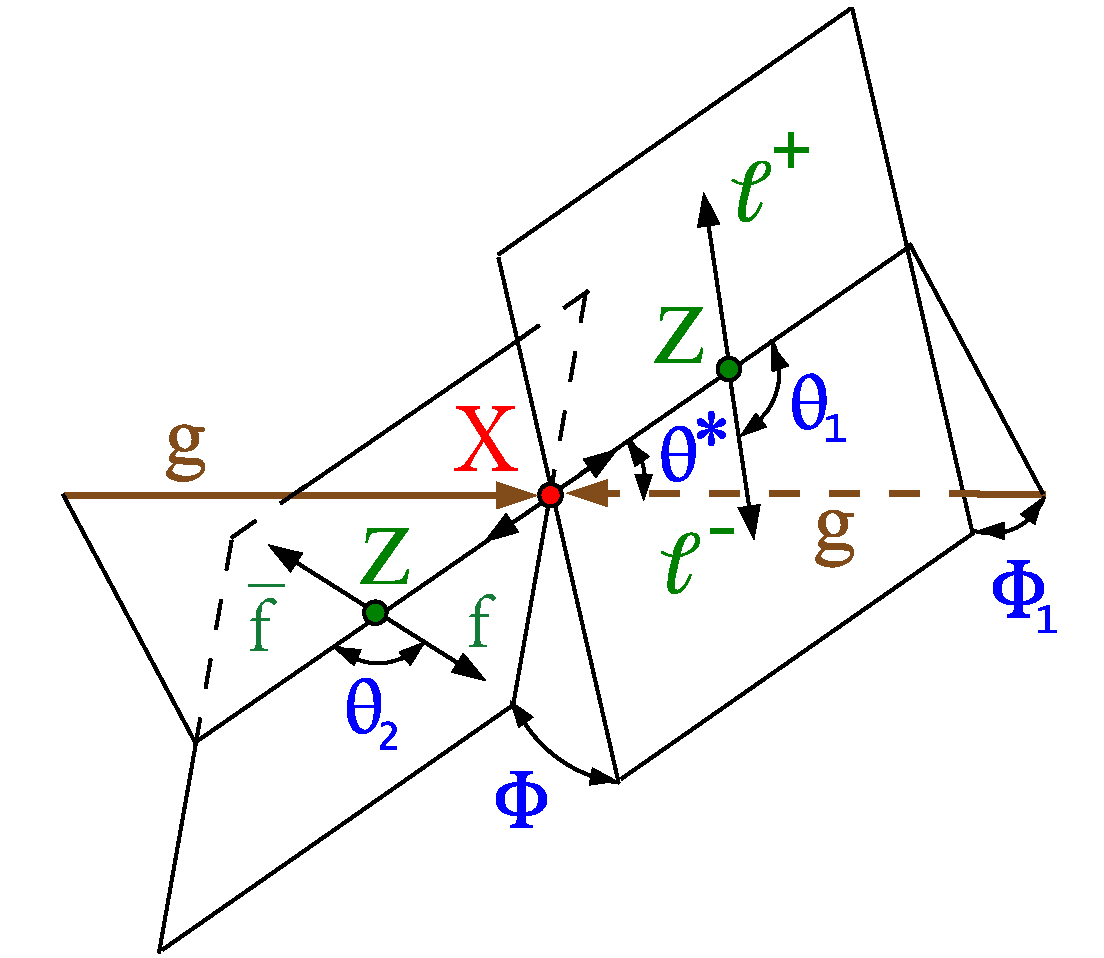
\includegraphics[width=0.45\textwidth]{figures/HighMassSearches/Figure_001-a.pdf}
    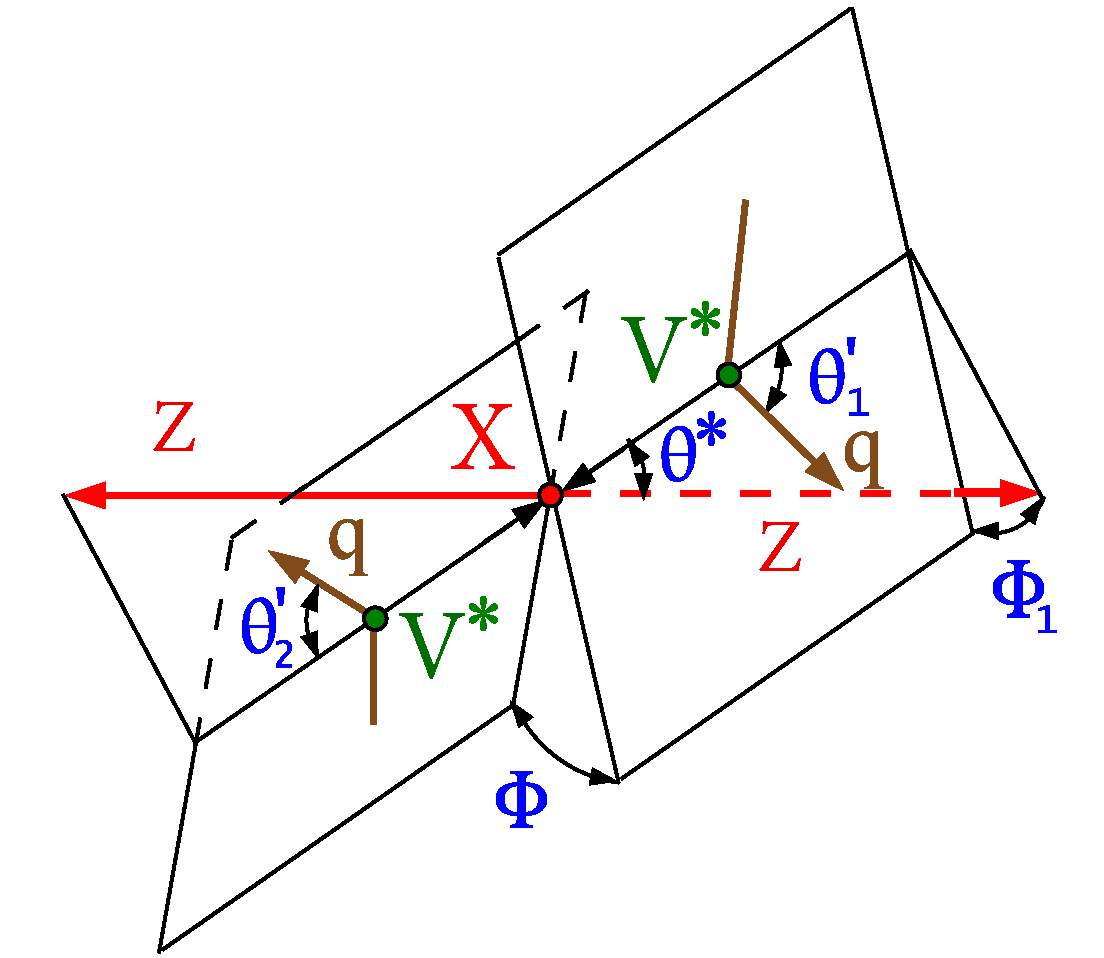
\includegraphics[width=0.45\textwidth]{figures/HighMassSearches/Figure_001-b.pdf}
    \caption
    {
    Illustration of an $\PX$ boson production from \ggF, $\Pg\Pg\to \PX\to \PZ\PZ\to (\ell^+\ell^-)(f\overline{f})$ (left), and VBF, $\Pq{\Pq^\prime}\to \Pq{\Pq^\prime} \PX \to \Pq{\Pq^\prime}\PZ\PZ$ (right). The five angles shown in blue and the invariant masses of the two vector bosons shown in green fully characterize either the production or the decay chain. The angles are defined in either the \PX\ or \PV\ boson rest frames~\cite{Gao:2010qx,Anderson:2013afp}.
    }
    \label{fig:decay}
\end{figure}

The discriminant sensitive to the $Z+JJ$ kinematics is calculated as
%%%%%%%%%%%%%%%%%%%%%
\begin{eqnarray}
\label{eq:Zjjmela}
\mathcal{D}_{\rm Zjj} =
\left[1+  \frac{  c_{\rm Zjj}\times{\cal P}_\text{Zjj} (\vec\Omega^{\PX\to2\ell2q} | m_{2\ell2q})}
{{\cal P}_{\PX\to2\ell2q} (\vec\Omega^{\PX\to2\ell2q} | m_{2\ell2q})} \right]^{-1}\,
\end{eqnarray}
%%%%%%%%%%%%%%%%%%%%%
where the denominator contains the probability of the signal
and the numerator includes the probability for the dominant $\PZ +jj$ background process,
all calculated either with the
$\JHUGEN{}$ (signal) or $\MCFM{}$ (background) matrix elements within the MELA framework.
The value of $c_{\rm Zjj}$ is tuned as a function of \mZZ{} in order to preserve good
the population of events in the range [0,1]. The template ${\cal T}(\mathcal{D}_{\rm Zjj}|m_{2\ell2q})$ used in the analysis is conditionally
normalised such that each slice of $\mathcal{D}_{\rm Zjj}$ is normalised to the unit area
for a given value of $m_{2\ell2q}$.

The discriminant sensitive to the VBF signal topology with two associated jets
is calculated as~\cite{Khachatryan:2015cwa, Khachatryan:2015mma}
%%%%%%%%%%%%%%%%%%%%%
\begin{eqnarray}
%
\label{eq:vbfmela}
\mathcal{D}_{2\rm jet} =
\left[1+
\frac{ c_{\rm XJJ}\times\mathcal{P}_{\rm XJJ} (\vec\Omega^{\rm \PX+JJ} | m_{2\ell2q}) }
{\mathcal{P}_{\rm VBF}  (\vec\Omega^{\rm \PX+JJ} | m_{2\ell2q})  }\right]^{-1}
\,,
%
\end{eqnarray}
%%%%%%%%%%%%%%%%%%%%%
where $\mathcal{P}_{\rm VBF}$ and $\mathcal{P}_{\rm \PX JJ}$ are probabilities obtained from the
\JHUGEN{} matrix elements for the VBF process and gluon fusion (technically a combination of
$gg/qg/qq^\prime$ parton collisions)
in association with two jets ($\PX+2$\,jets) within the MELA framework.
The value of $c_{\rm XJJj}$ is tuned as a function of mass to preserve good
the population of events in the range [0,1]. This discriminant help us in discriminating the VBF/ggH topology.

\section{Event reconstruction and selection}
\label{sec:EventSelection}
% This is my fig.~\ref{fig:test}.
% \begin{figure}[!htb]
%     \centering
%     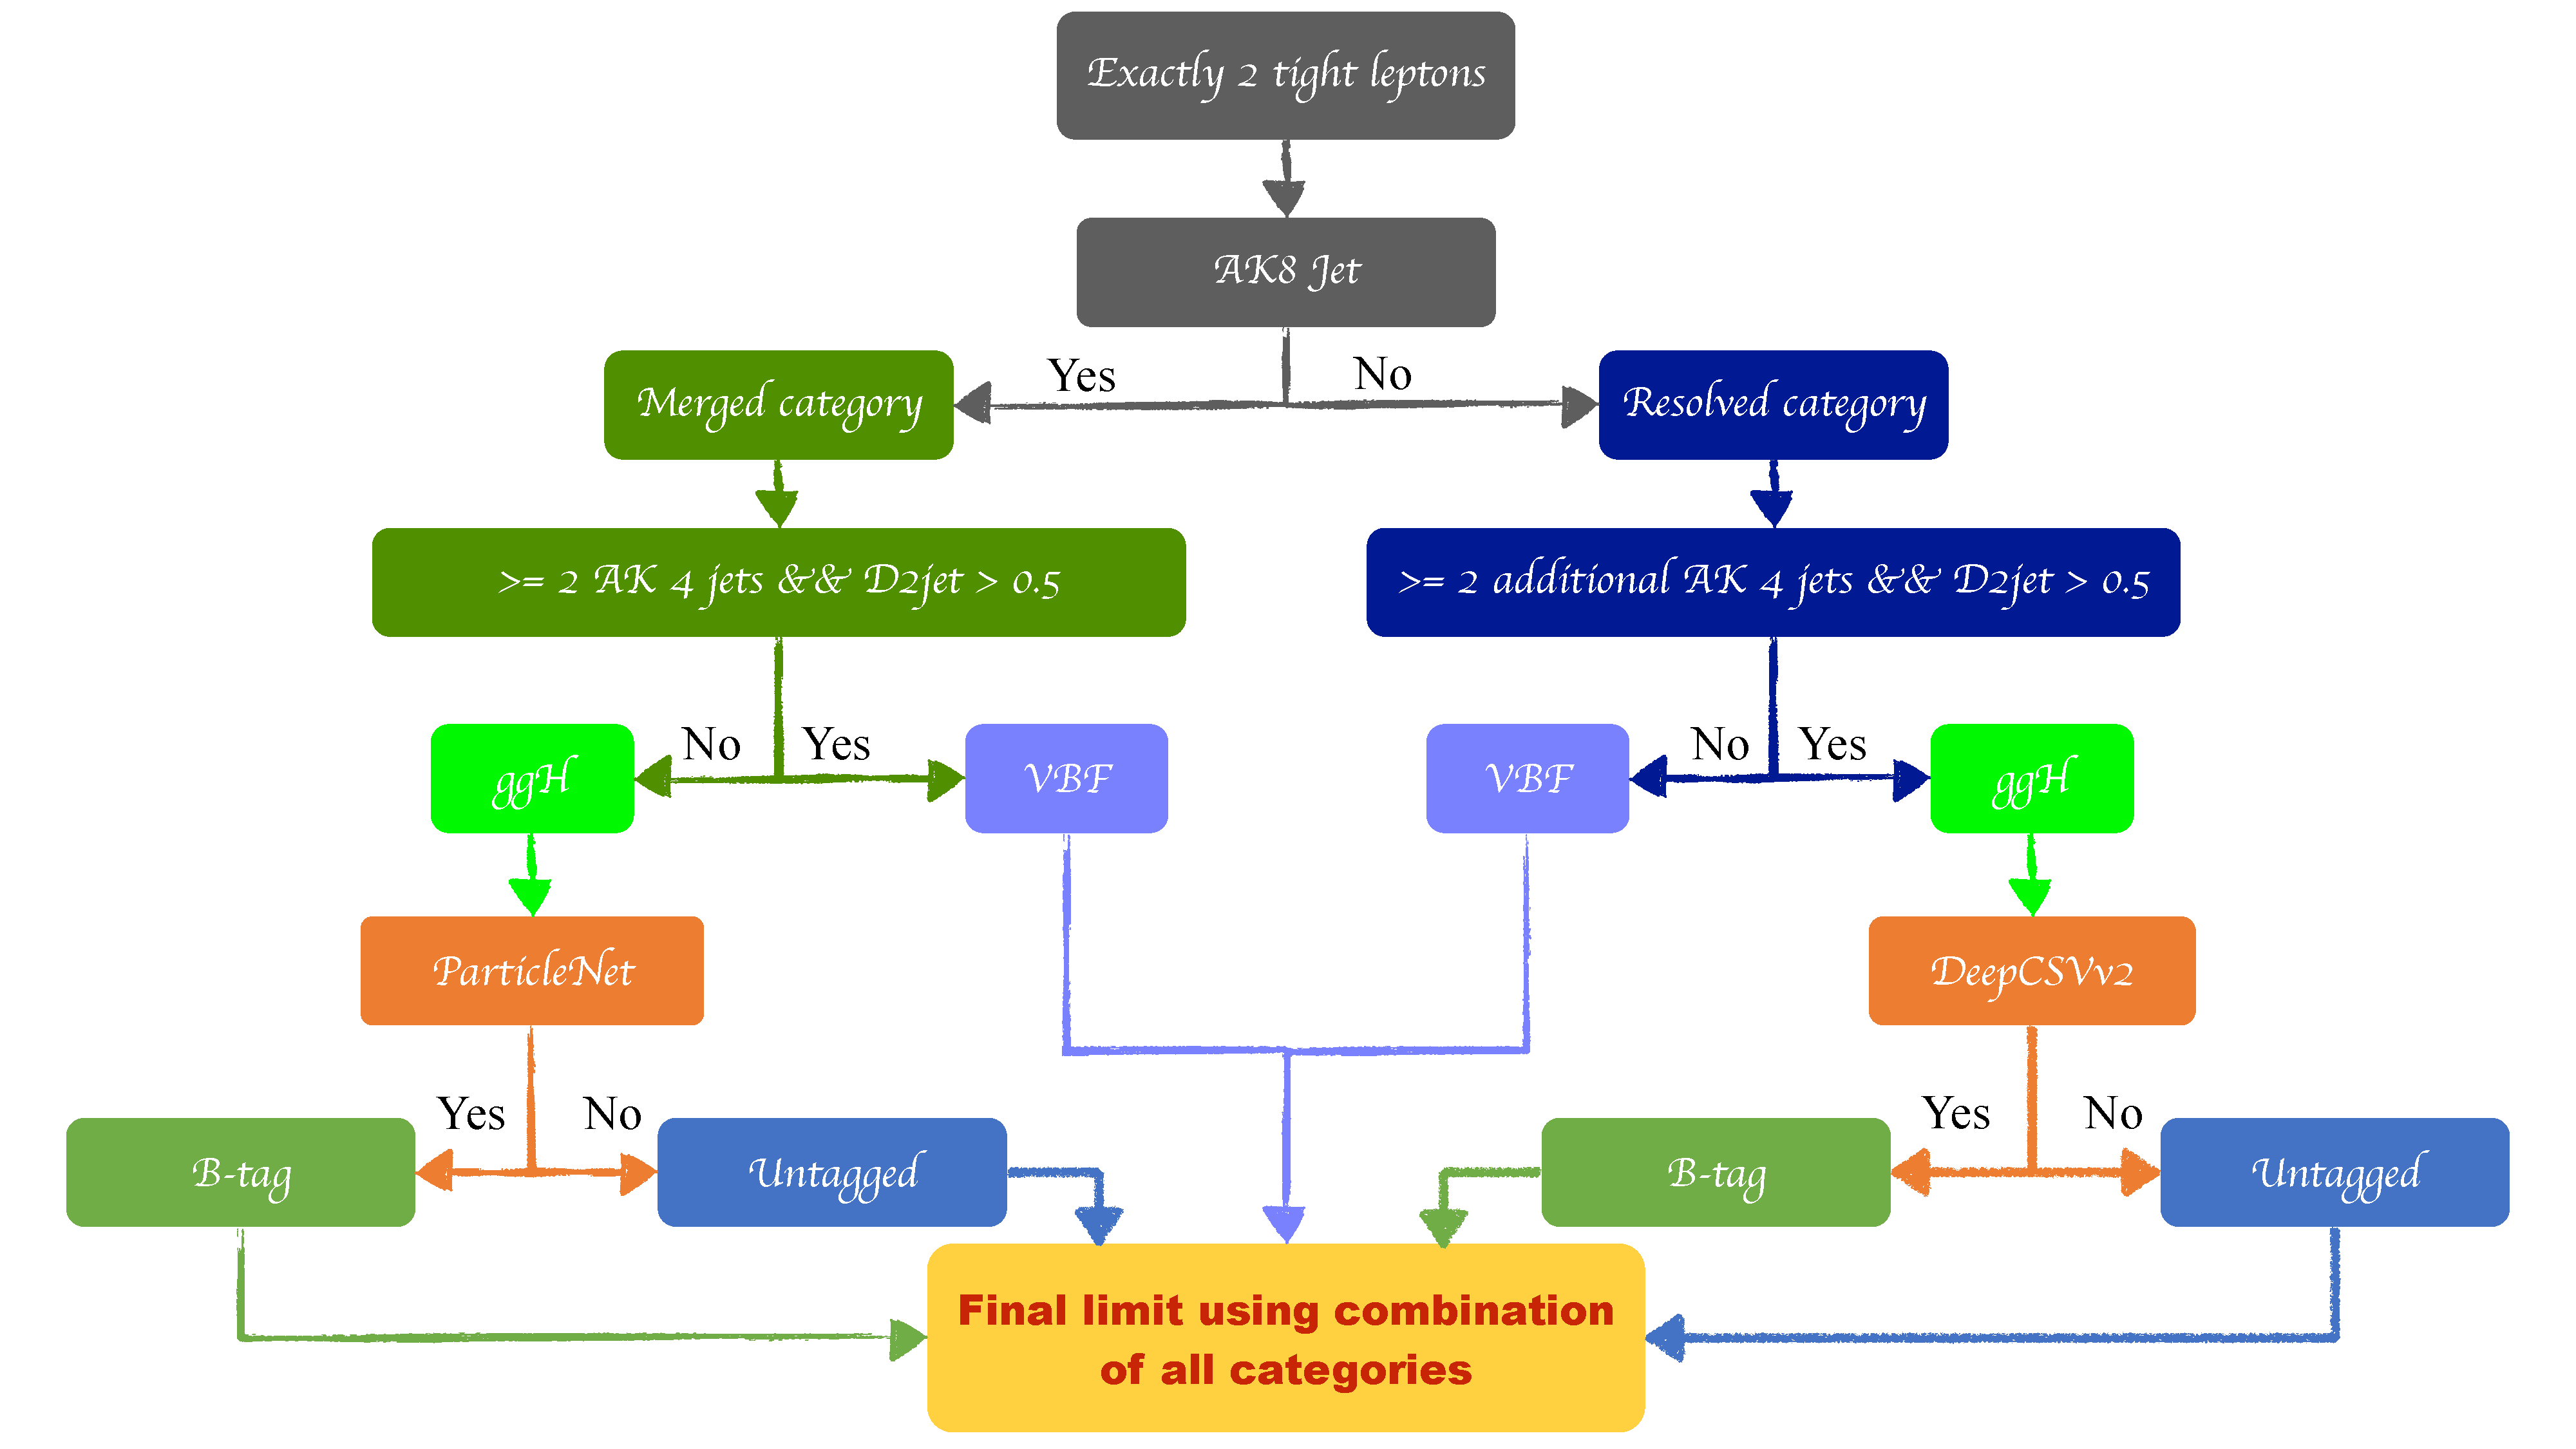
\includegraphics[width=\textwidth]{figures/HighMassSearches/ZZ2l2Q_FlowChart.pdf}
%     \caption[Caption for TOC]{Even selection flow chart.}
%     \label{fig:test}
% \end{figure}
%
In the CMS detector, the Particle-Flow (PF) algorithm~\cite{Sirunyan:2017ulk} is employed to reconstruct and identify individual particles as charged and neutral hadrons, leptons, and photons by combining information from all sub-detectors.
The primary vertex (PV) is defined as the vertex with the highest sum of squared transverse momenta from charged tracks.

The leptons considered are required to be associated with the PV of the event~\cite{Chatrchyan:2014fea} to suppress electron candidates originating from photon conversions and lepton candidates from in-flight decays of heavy quarks.
Additionally, leptons must be isolated from other particles in the event.
This analysis selects tight electrons or muons, defined as PF electrons or muons that pass a tight identification requirement, with an average efficiency of approximately 90%\todo{Check this number}.

An algorithm is used to recover the final state radiation (FSR) from leptons.
Photons reconstructed by the PF algorithm are considered as FSR candidates if they satisfy specific criteria, $\PT^{\Pgg} > 2\GeV$ and ${\cal I}^{\ell}< 1.8$~\cite{Sirunyan:2017exp}, and those that do not satisfy additional requirements are discarded.
The lowest candidate for every lepton is retained, and the photons identified as FSR are excluded from any isolation computations.

In addition to ID requirements, leading and sub-leading lepton candidates must have transverse momenta greater than 40 and 24 GeV, respectively, and a pseudorapidity in the range (0 $<$ $|\eta|$ $<$ 2.4), to remain in the CMS tracker region.

Jets are constructed using the anti-kT clustering method and are required to pass a loose identification criteria to reject jets from pileup interactions~\cite{antikt,Cacciari:2011ma}.
The considered jets should satisfy certain conditions and be separated from all selected leptons by a $\Delta R(\ell,\text{jet})>0.4$.
The analysis uses b-tagged jets, having $\abs{\eta^{\text{jet}}}<2.4$, for event categorization and selection, where a b-jet is tagged using the deep combined secondary vertex algorithm based on the impact parameter significance of the tracks associated with the jet~\cite{Chatrchyan:2012jua,CMS-PAS-BTV-15-001}. The loose working point is used, corresponding to an efficiency of 80\% and a mistag rate of 10\% for light quark jets.

The main feature distinguishing the two dominant $\PX$ boson production mechanisms (\ggF and VBF) is the presence of associated jets and the kinematic correlation between such jets and the $\PX$ boson.
Events are split into categories based on kinematic correlations to gain sensitivity to the production process of the $\PX$ boson.
A ME technique is employed to categorize events based on the correlation between the two forward jets and the $\PX$ boson candidate.
In this analysis, events are selected by combining leptonically and hadronically decaying \cPZ\ candidates.

The $\cPZ$ candidates are formed from pairs of leptons of the same flavor and opposite charge ($\Pe^{+}\Pe^{-}$, $\Pgm^{+}\Pgm^{-}$) and are required to pass the invariant mass selection $60 < m_{\ell^+\ell^-} < 120\GeV$.
A minimum dilepton transverse momentum, \PT{} of \unit{\DILEPTONPTCUT}{\GeV}, is imposed to reject Drell-Yan events with small hadronic recoil.

Hadronically decaying $\cPZ$ boson candidates (\Zhad) are reconstructed using two distinct techniques, referred to as "resolved" and "merged."
In the resolved case, the two quarks from the $\cPZ$ boson decay form two distinguishable AK4 jets, while in the merged case, a single AK8 jet with a large transverse momentum is taken as a \Zhad.

In the merged jet case, a pruning algorithm is applied to the AK8 jet to recluster the jet constituents while applying additional requirements that eliminate soft, large-angle QCD radiation that artificially increases the jet mass relative to the nominal $\cPZ$ boson mass~\cite{prune,substructure}.

Jets must not overlap with leptons, so a cut on $\Delta R(\ell, jet) > 0.4~(0.8\textrm{~for merged})$ is applied to resolved and merged jets.
Finally, the reconstructed events are required to have an invariant mass around the $\cPZ$ boson mass: $\LSBLOW < \MZhad < \unit{\USBHIGH}{\GeV}$.
Among this, the region 70--105 GeV is considered the signal region, while the regions 40--70 GeV and 135--180 GeV form the sideband region.
The region with possible $\Ho \to \bbbar$ signals, 105--135 GeV, is removed from any selection.
Furthermore, a $\PT > \unit{\VHADRESOLVEDPTCUT}\ (\VHADMERGEDPTCUT) {\GeV}$ is applied in the resolved (merged) case.
Finally, we consider events with $m(\ell\ell J) > 100$ GeV.%\todo{Check the mZZ cut}

To minimise contamination from standard model DY + jets production and QCD, we further require that the hadronic Z boson candidate from a merged selection has a substructure.
The ParticleNet tagger is exploited to ensure that the candidate has substructure.

The selection preference is given to merged jets when multiple categories are present. If no merged jets are found, the resolved category is considered.
Within each selection category, the candidate with the largest transverse momentum has priority over the others.

The hadronically and leptonically decaying $\cPZ$ boson candidates are combined to form a resonance candidate.
The reconstructed $\cPZ\cPZ$ candidate mass (\mZZ{}) denotes the dilepton + dijet mass (\mlljj{}) in the resolved case and the dilepton + merged jet invariant mass (\mllJ{}) in the merged case.
A requirement of $\mZZ{}> \unit{\MZZCUT}{\GeV}$ is imposed to reduce the $\cPZ + \text{jets}$ background.%\todo{Check}

To increase sensitivity to different production modes, events are categorized into VBF and inclusive types.
Furthermore, a dedicated category is defined for events enriched with \cPqb\ quark jets due to the presence of $\cPZ\to\bbbar$ decays. The definitions are as follows:
\begin{itemize}
	\item  \textbf{VBF-tagged} requires two additional and forward jets besides those constituting the hadronic $\cPZ$ boson candidate; a mass dependent selection criterion on ${\cal D}^\mathrm{VBF}_{\mathrm{2jet}}$ is applied;
	\item  \textbf{\cPqb\ tagged} consists of the remaining events with two \cPqb\ tagged jets (in the resolved case) or two \cPqb\ tagged subjets from the hadronic $\cPZ$ boson candidate;
	\item  \textbf{Untagged} consists of the remaining events.
\end{itemize}

As a result of this categorization, events are split into twelve categories: $2\Pe 2\Pq$ or $2\mu 2\Pq$, either VBF-tagged, b-tagged, or untagged, and each with either merged jets or resolved jets.
Each event is characterized by the two observables ($\mZZ$, $\ZJJMELA$). The invariant mass distribution for merged and resolved events in each category after the selection is shown in Fig~\ref{fig:ZZmass_untag}. The \ZJJMELA and \VBFMELA distributions for resolved events in each category together after the selection are shown in Fig.~\ref{fig:ZZmela_untag}.

\begin{figure}[htbp]
    \centering
    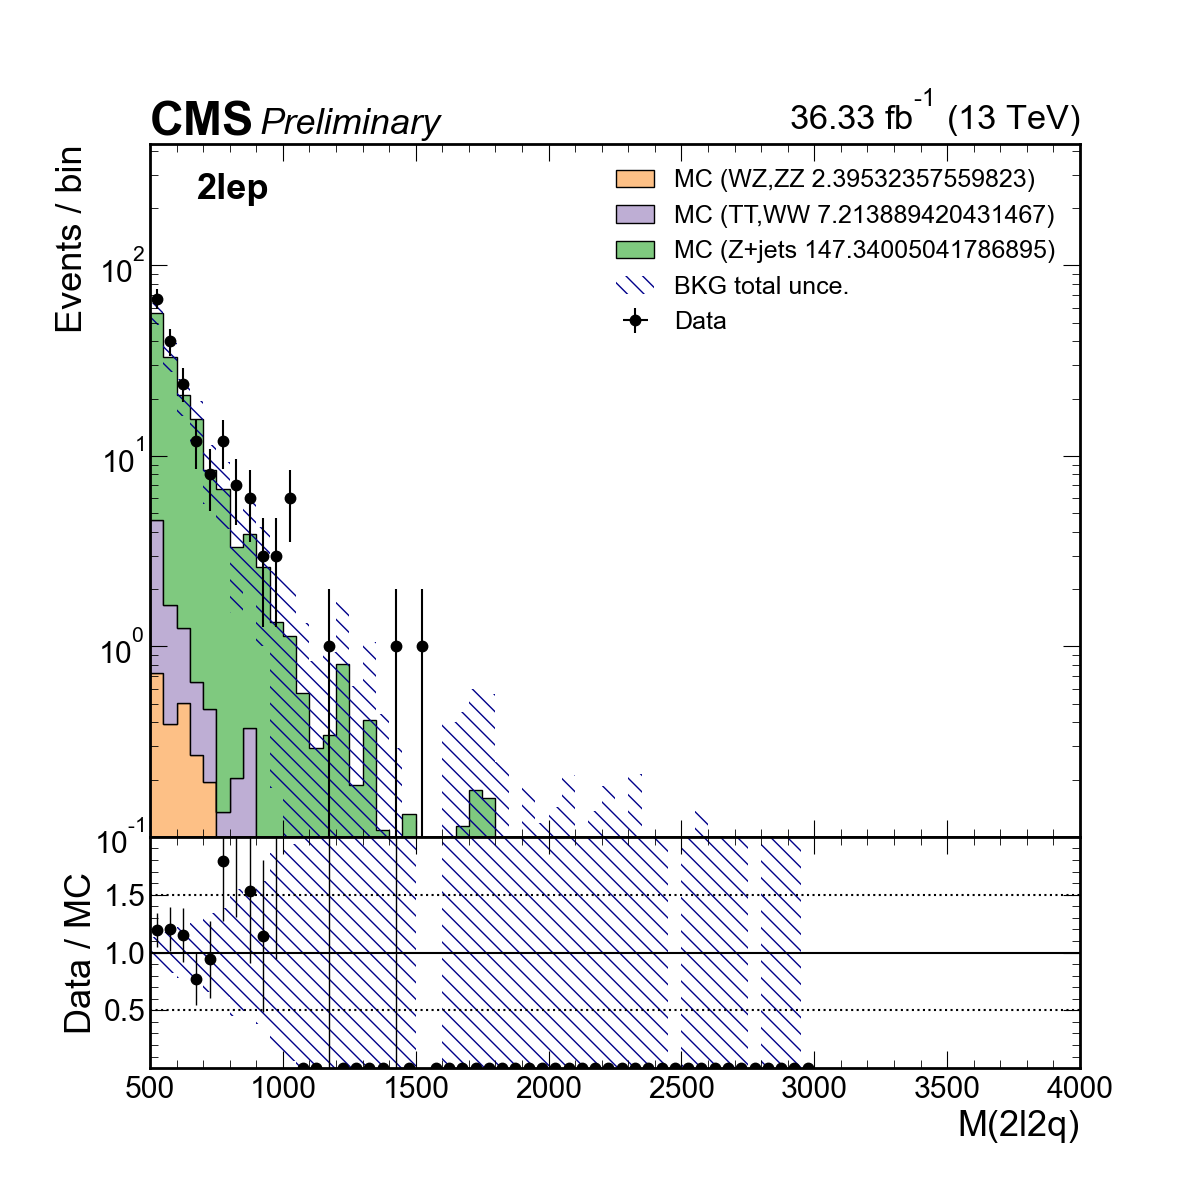
\includegraphics[width=0.45\textwidth]{figures/HighMassSearches/dataMCPlots/mass2l2jet_CR_2lep_btag.png}
    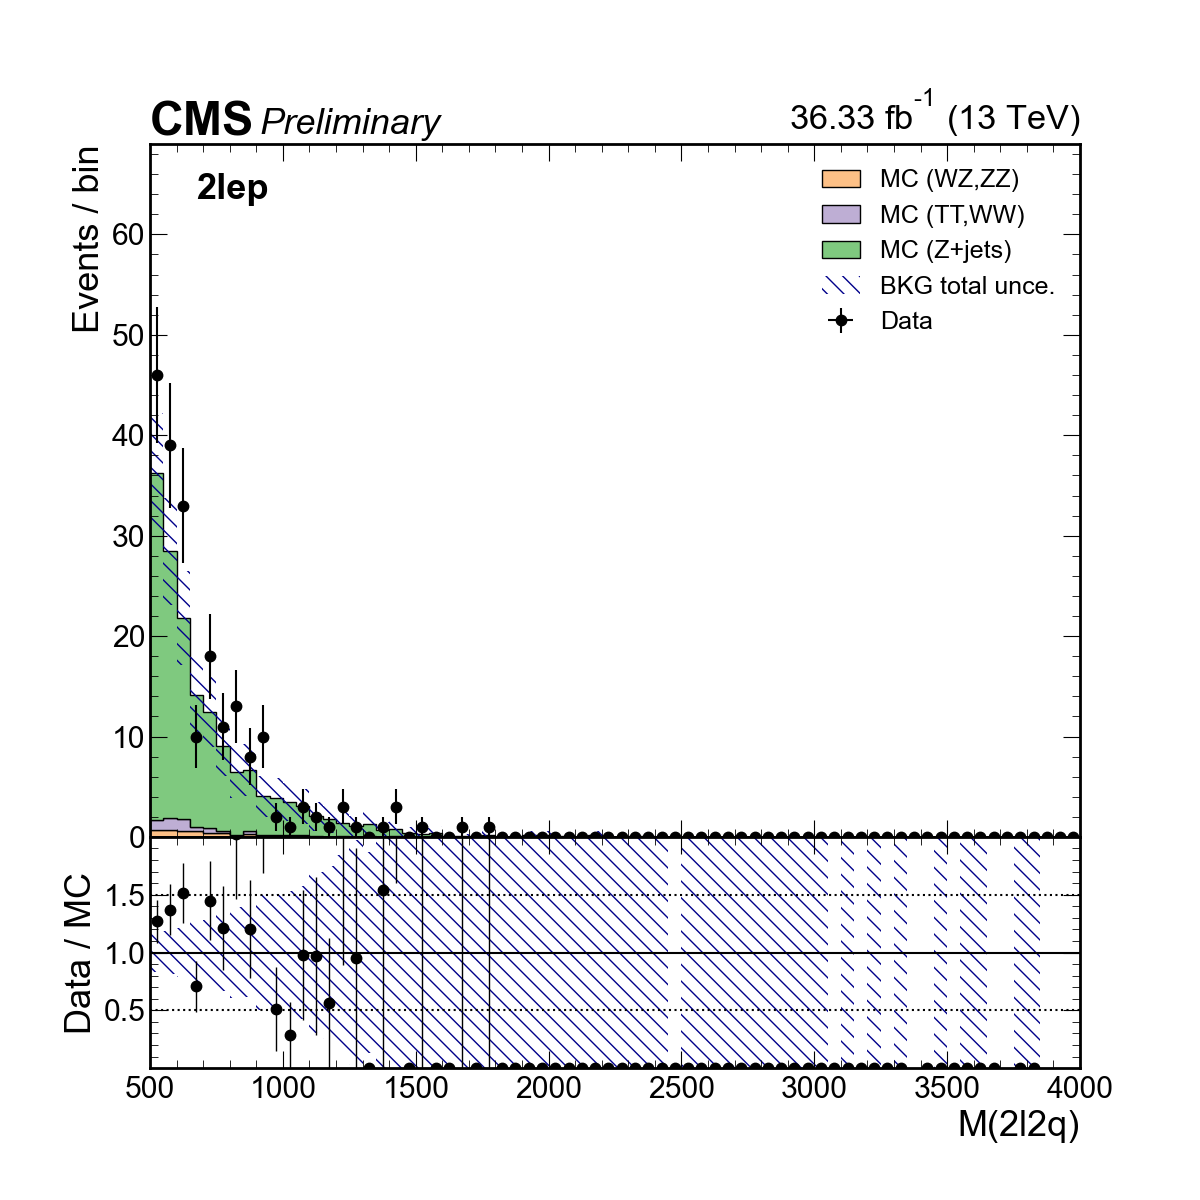
\includegraphics[width=0.45\textwidth]{figures/HighMassSearches/dataMCPlots/mass2lj_CR_2lep_btag.png}\\
    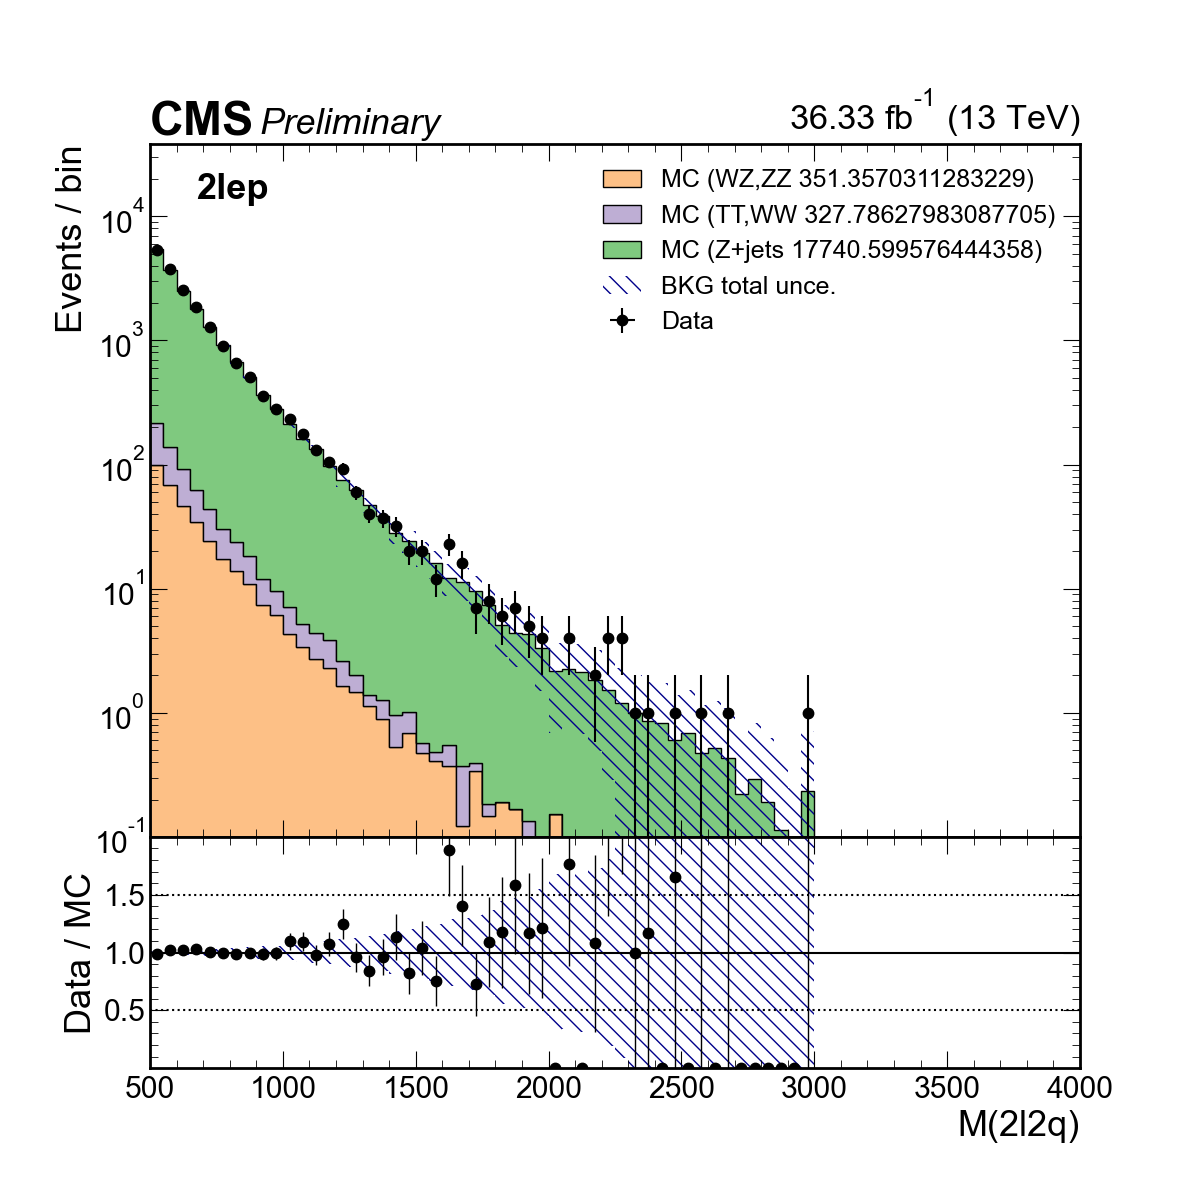
\includegraphics[width=0.45\textwidth]{figures/HighMassSearches/dataMCPlots/mass2l2jet_CR_2lep_untag.png}
    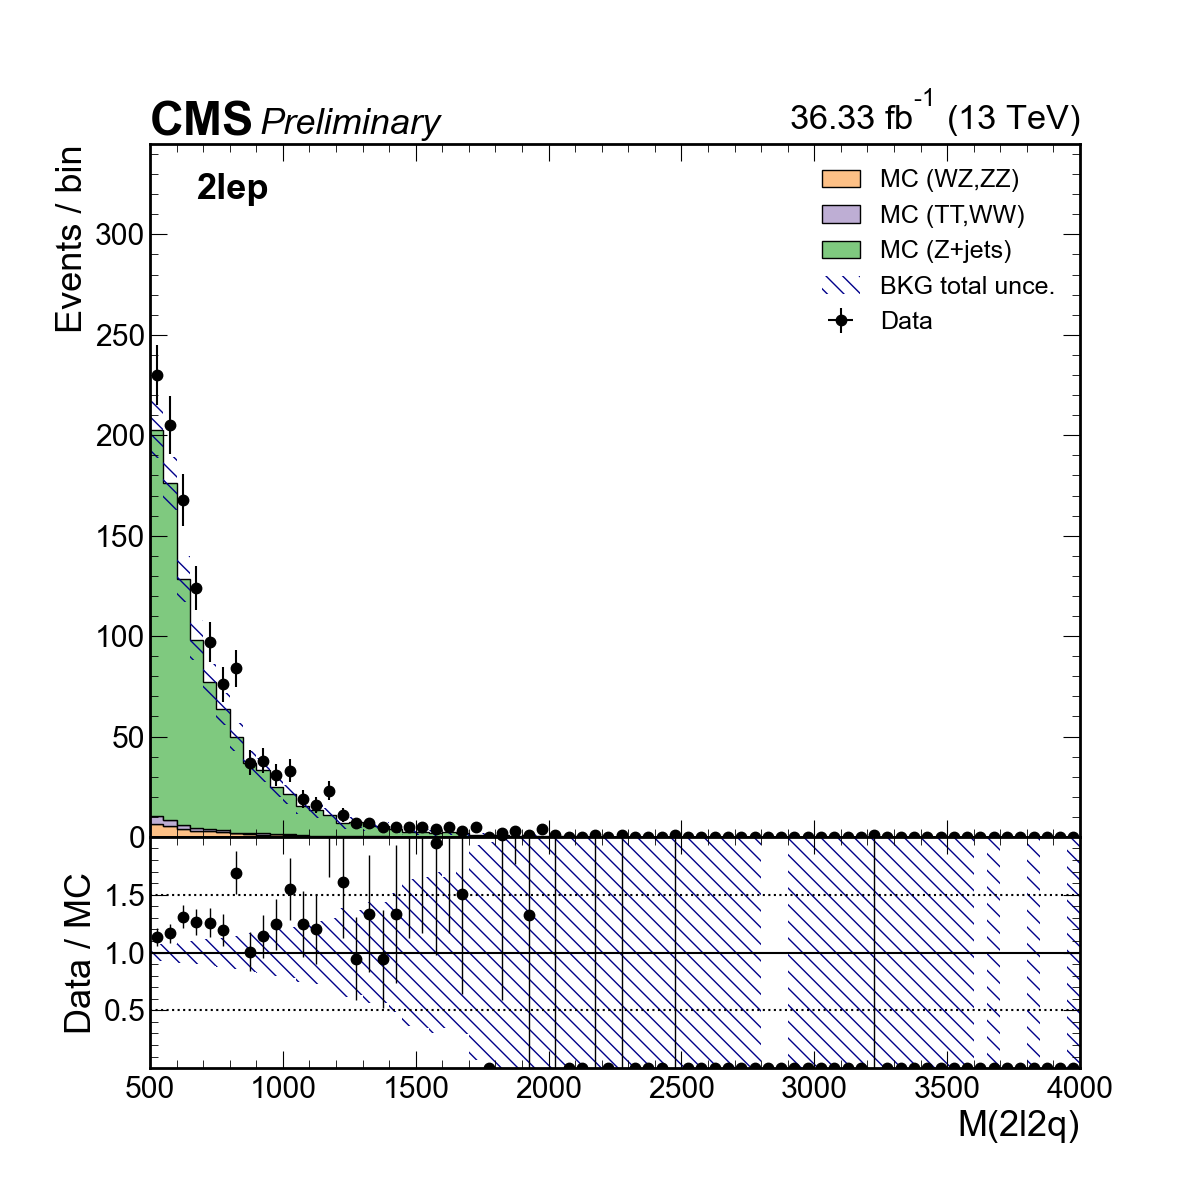
\includegraphics[width=0.45\textwidth]{figures/HighMassSearches/dataMCPlots/mass2lj_CR_2lep_untag.png}
    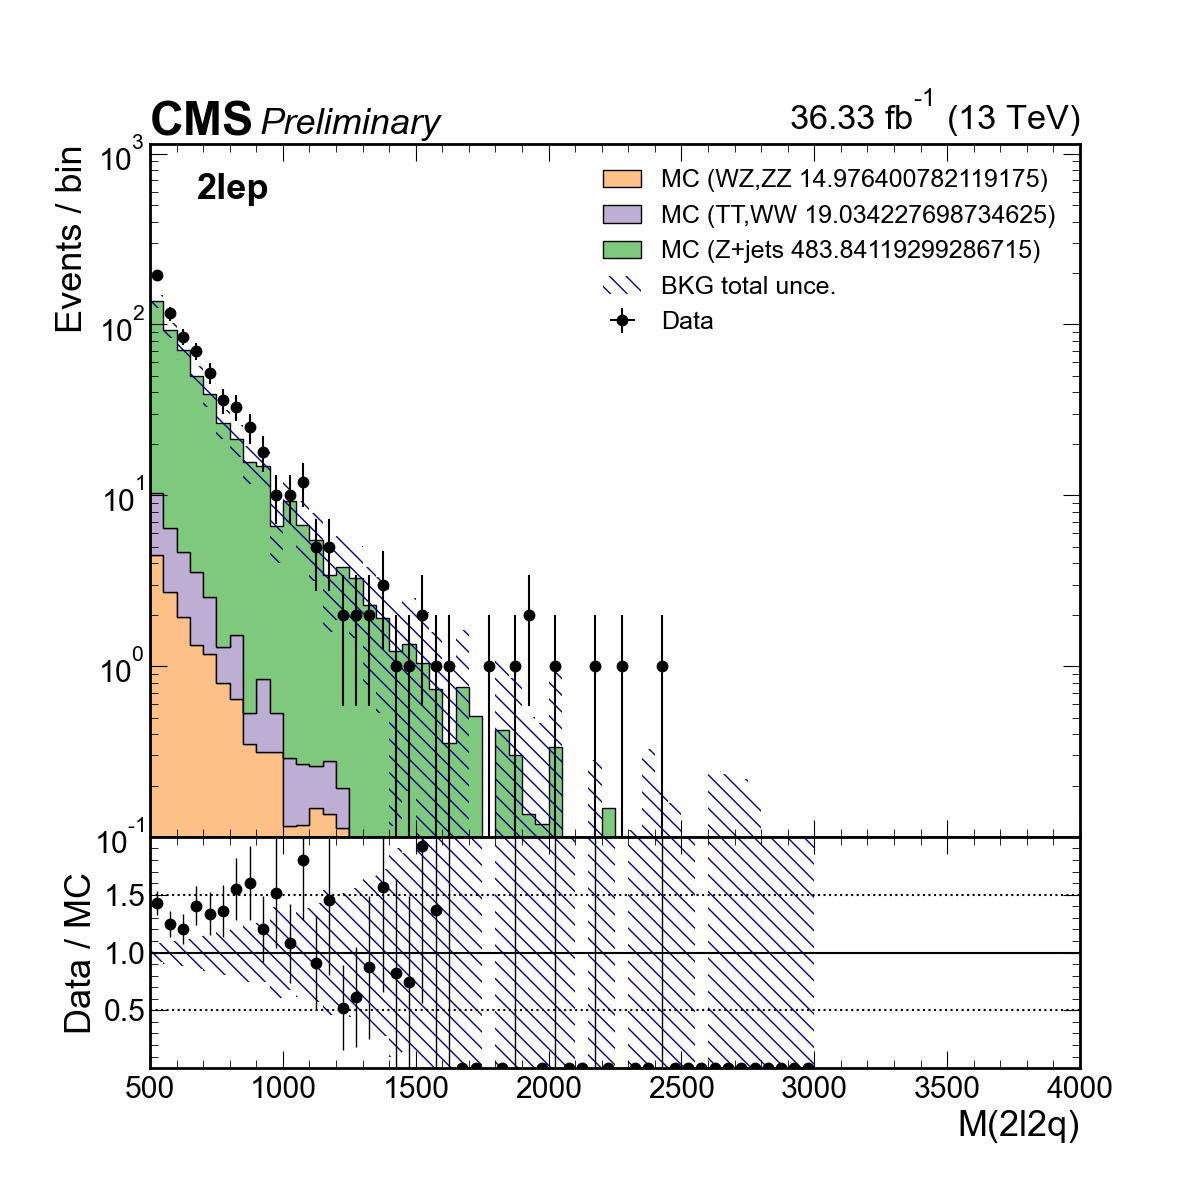
\includegraphics[width=0.45\textwidth]{figures/HighMassSearches/dataMCPlots/mass2l2jet_CR_2lep_vbftag.png}
    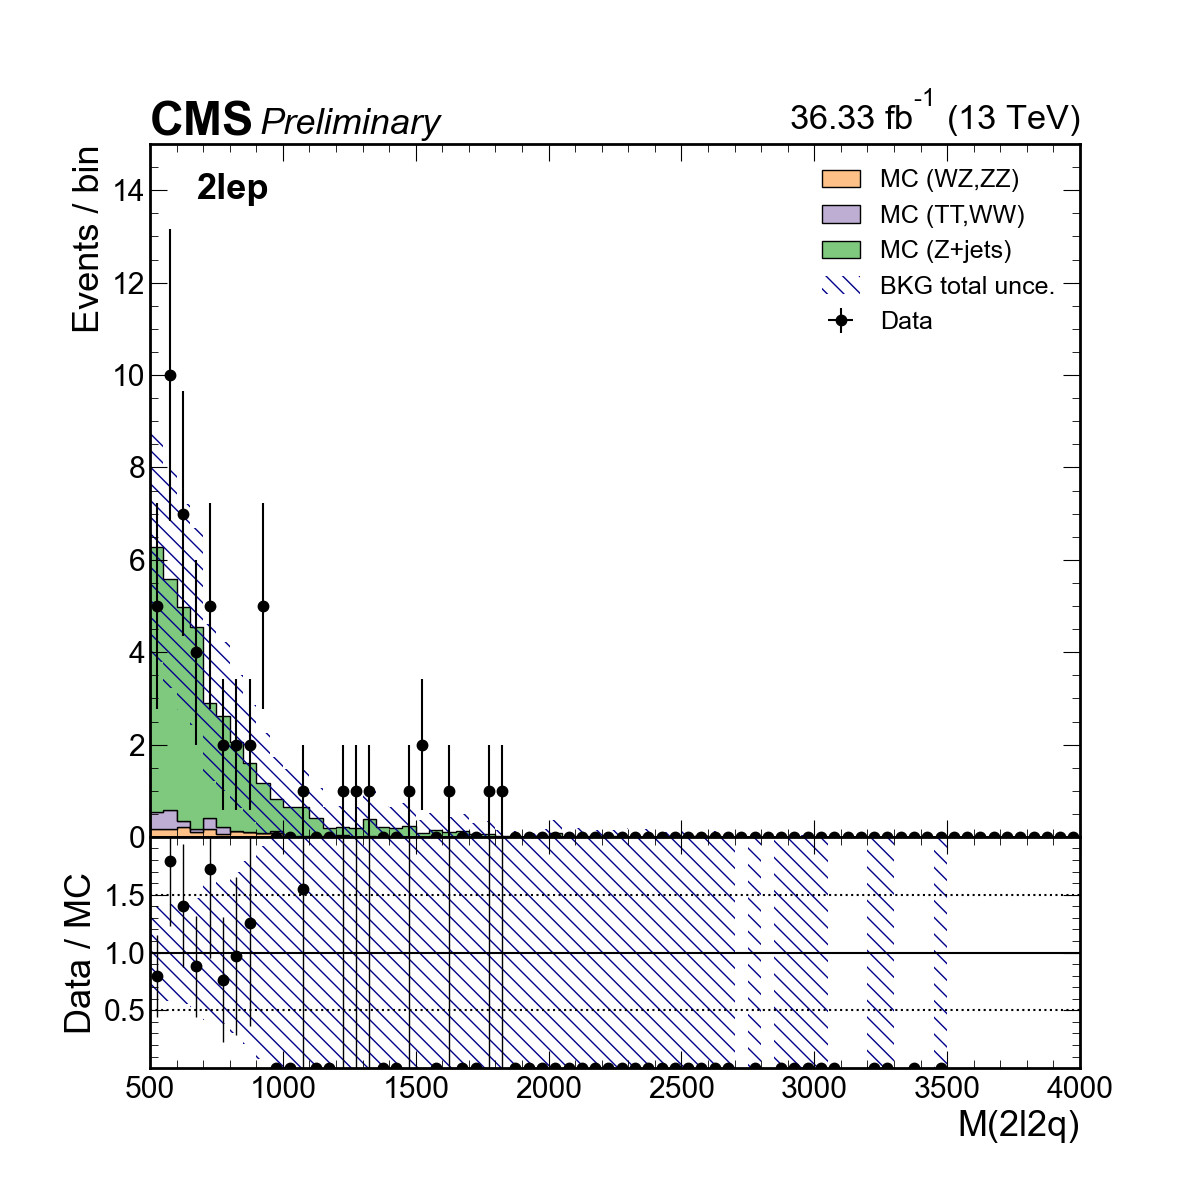
\includegraphics[width=0.45\textwidth]{figures/HighMassSearches/dataMCPlots/mass2lj_CR_2lep_vbftag.png}\\

    \caption{Distributions of the invariant mass \mZZ{} in the control region for the merged (right) and resolved (left) case for the different categories in the $2{\ell}2\Pq$ channel for 2016.
    % The points represent the data, the stacked histograms the expected backgrounds from simulation, and the open histograms the expected signal. The blue hatched bands refer to the sum of background estimates derived from either simulation or control samples in data, as described in the text.
    Lower panels show the ratio between data and background estimation in each case.
    }
    \label{fig:ZZmass_untag}
 \end{figure}

 \begin{figure}[htbp]
    \centering
    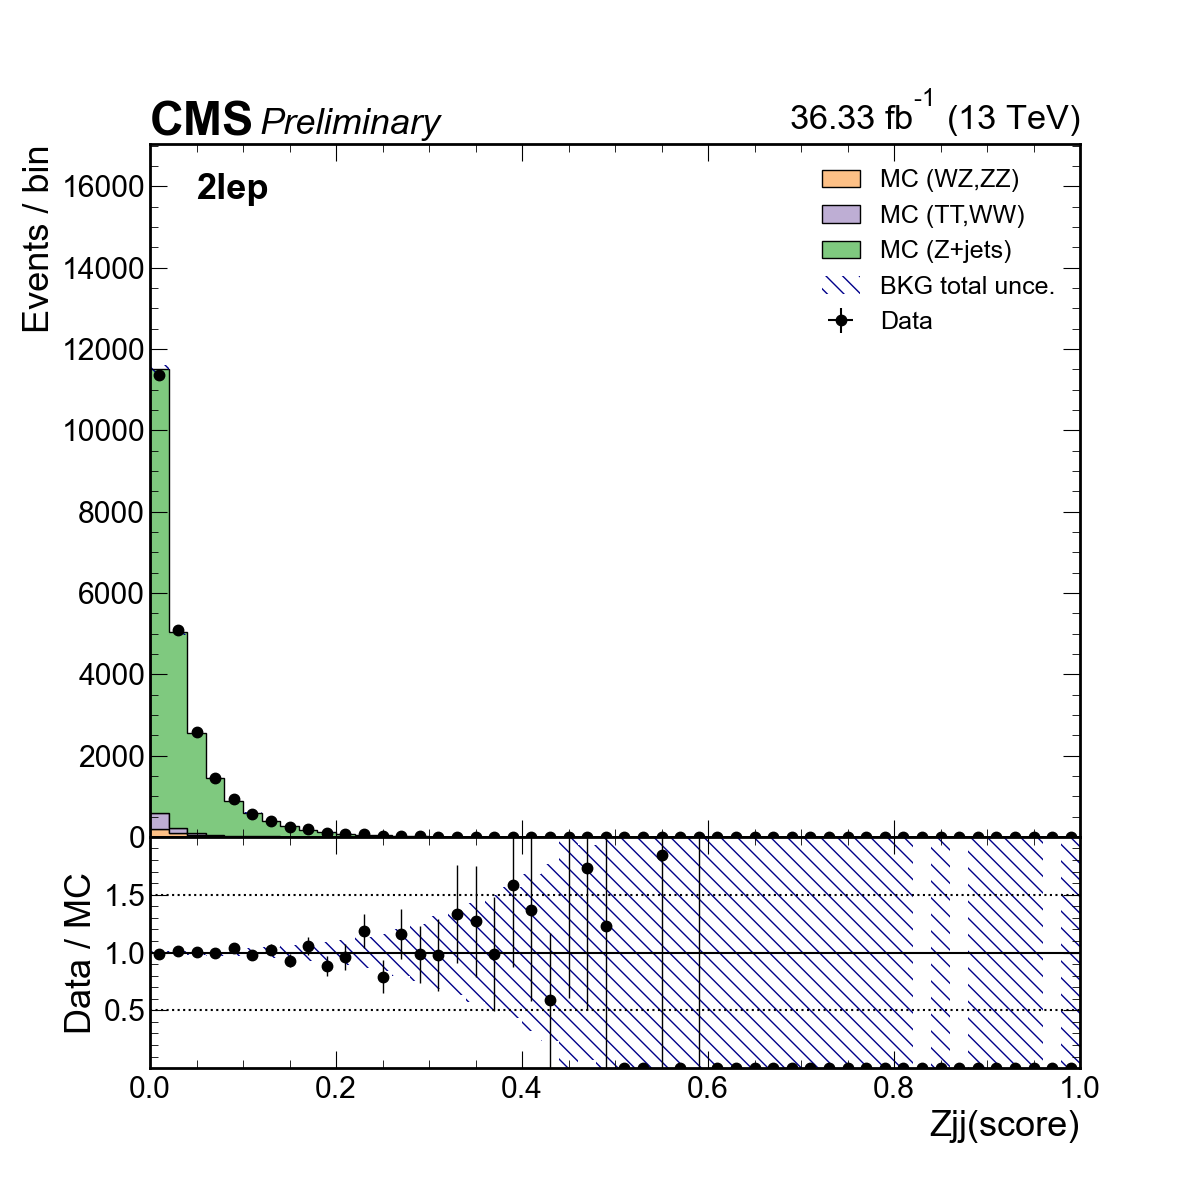
\includegraphics[width=0.45\textwidth]{figures/HighMassSearches/dataMCPlots/KD_ZJ_2lep.png}
    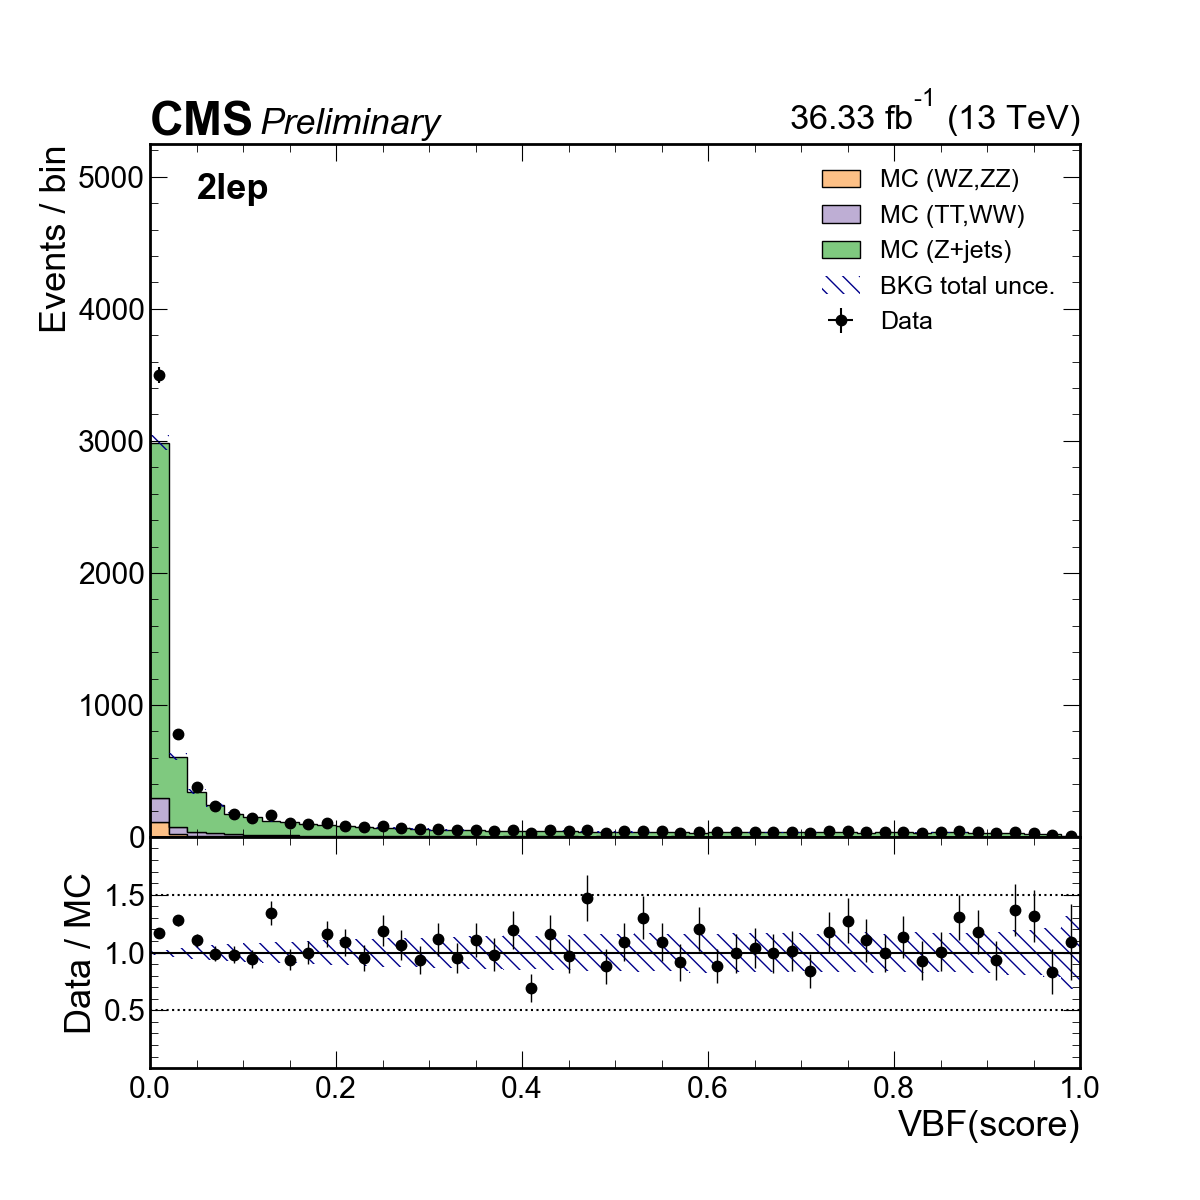
\includegraphics[width=0.45\textwidth]{figures/HighMassSearches/dataMCPlots/KD_JVBF_2lep.png}\\
    \caption{Distributions of the \ZJJMELA (left) and \VBFMELA (right) discriminants in the control region for the merged selection. The points represent the data, the stacked histograms the expected background from simulation.
    % , and the open histograms the expected signal.
    }
    \label{fig:ZZmela_untag}
 \end{figure}

 \section{Signal and background parameterization}
 \label{Section_parameterization}

 The goal of the analysis is to determine if a set of $\PX$ boson parameters
 $\mX$, $\GX$, and $\sigma_i\mathcal{B}_{X\to\cPZ\cPZ}$ is consistent with the data, where $\sigma_i\mathcal{B}_{X\to\cPZ\cPZ}$ is the product of the signal production cross section and
 the $\PX\to\cPZ\cPZ$ branching fraction in each production channel $i$ (gluon fusion or EW production). In practice, the $\sigma_i\mathcal{B}$ for $i=1,2$ are expressed in terms of
 $\sigma_{\mathrm{tot}}\mathcal{B}_{X\to\cPZ\cPZ}$ and $f_{\mathrm{VBF}}$, where $\sigma_{\mathrm{tot}}$ is the sum of the cross sections in the two production channels. The confidence intervals on $\sigma_{\mathrm{tot}}\mathcal{B}_{X\to\cPZ\cPZ}$
 are determined from profile likelihood scans for a given set of parameters $(\mX, \GX, f_{\mathrm{VBF}})$.
 The extended likelihood function is defined for candidate events as
 \begin{eqnarray}
 \mathcal{L} =  \exp\Big( - \sum_{i} n_{vv}^i -\sum_i n_\text{bkg}^i  \Big)
 \prod_k \prod_j
 \Big(
   \sum_i n_{vv}^{i} \mathcal{P}^{i,k}_{vv}(\vec{x}_{j}; \mX, \GX)
 +\sum_i n_\text{bkg}^{i} \mathcal{P}^{i,k}_\text{bkg}(\vec{x}_{j})
 \Big),
 \label{eq:likelihood}
 \end{eqnarray}
 where $n_{vv}^i$ and $n_\text{bkg}^i$ are the numbers of signal and background events in channel $i$. The observables $\vec{x}_j$ are defined for each event $j$ in category $k$.
 % as discussed in Sections~\ref{sec:XZZ4l}, \ref{sec:XZZ2l2q}, and~\ref{sec:XZZ2l2nu}.
 There are several signal and background types~$i$, defined for each production mechanism.
 The background processes that do not interfere with the signal are described by the probability density functions (pdfs)
  $\mathcal{P}^{i,k}_\text{bkg}(\vec{x}_{j})$. The $vv\to \ff$ process is described by the pdf
 $\mathcal{P}^{i,k}_{vv}(\vec{x}_{j}; \mX, \GX)$ for $vv=\Pg\Pg$ (gluon fusion) and $vv= $ VV (EW production).
 This pdf describes the production and decay of the $\PX$ boson signal, SM background, including $\PH(125)$, and interference between all these contributions
 and is parameterized as follows:
 \begin{eqnarray}
 \mathcal{P}^{i,k}_{vv} (\vec{x}_{j}; \mX, \GX) =
 \mu_i  \mathcal{P}^{i,k}_{vv\to \PX\to \ff} (\vec{x}_{j}; \mX, \GX)
 + \sqrt{\mu_i}  \mathcal{P}^{i,k}_{\mathrm{int}} (\vec{x}_{j}; \mX, \GX)
 + \mathcal{P}^{i,k}_{vv\to\ff} (\vec{x}_{j})
 ,
 \label{eq:psig}
 \end{eqnarray}
 where $\mu_i$ is the relative signal strength for production type $i$ defined as the ratio of
 $\sigma_i\mathcal{B}$ with respect to a reference value, for which normalization of the pdf is determined.
 The interference contribution $\mathcal{P}^{i,k}_{\mathrm{int}}$ scales as $\sqrt{\smash[b]{\mu_i}}$ and the pure signal as ${\mu_i}$,
 while both depend on the signal parameters $\mX$ and $\GX$.
 The likelihood defined in Eq.~(\ref{eq:likelihood}) is maximized with respect to the nuisance parameters,
 which include the constrained parameters describing the systematic uncertainties.

 \subsection{Signal model}
 \label{sec:Signalmodel}

 The parameterization of $\mathcal{P}^{i,k}_{vv} (\vec{x}_{j}; \mX, \GX)$ is performed using the MC simulation
 discussed in Section~\ref{sec:MC} with the ME method.

 We parameterize the signal mass shape as follows:
 A pdf after detector effects ${\cal M}^{\mathrm{reco}}_{vv}(m_{\cPZ\cPZ})$ is implemented with the multiplicative efficiency function  ${\cal E}(m_{\cPZ\cPZ})$ and convolved with a mass resolution function
 ${\cal R}(m_{\cPZ\cPZ}|m^{\mathrm{Gen}}_{\cPZ\cPZ})$, both extracted from simulation of the \ggF and VBF processes:

 \begin{eqnarray}
 {\cal M}^{\mathrm{reco}}_{vv}(m_{\cPZ\cPZ})=
 \left({\cal E}(m_{\cPZ\cPZ}^{\mathrm{Gen}}) {\cal M}_{vv}(m^{\mathrm{Gen}}_{\cPZ\cPZ}|\mX,\GX)\right) \otimes {\cal R}(m_{\cPZ\cPZ}|m^{\mathrm{Gen}}_{\cPZ\cPZ}).
 \label{eq:signalpdf1D}
 \end{eqnarray}

 The parameterizations of ${\cal R}(m_{\cPZ\cPZ}|m^{\mathrm{Gen}}_{\cPZ\cPZ})$ and ${\cal E}(m_{\cPZ\cPZ}^{\mathrm{Gen}})$ cover the mass
 range from 500\GeV to 3\TeV. Figure~\ref{fig:eff} shows the efficiencies in the various categories. The resolution is 3--5\%. With the above ingredients, the $m_{\cPZ\cPZ}$ parameterization is shown in Fig.~\ref{fig:mzz_interference}, for a boson with $\mX = 500\GeV$, $\GX = 15\GeV$.
 % The interference contributions from $\PH(125)$ and $\Pg\Pg\to\cPZ\cPZ$ background are also shown.

 \begin{figure}[htbp]
 \centering
 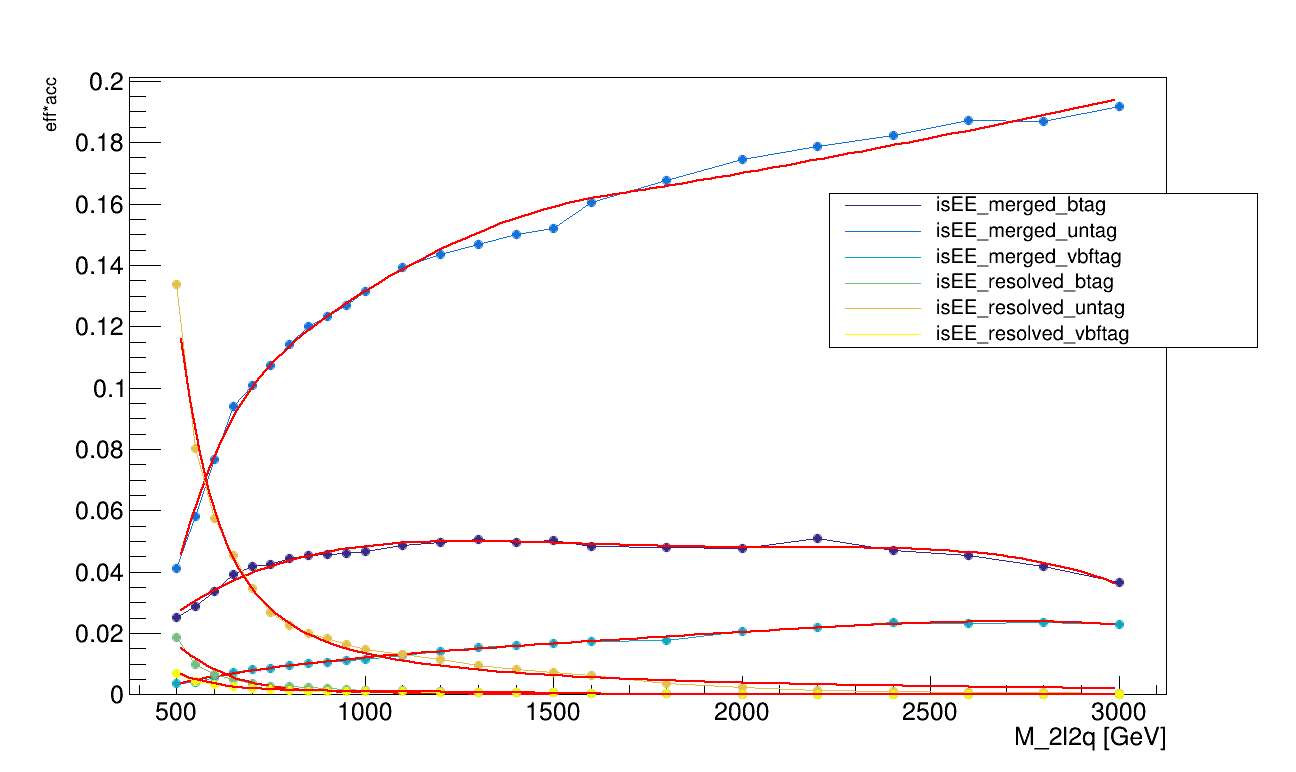
\includegraphics[width=0.45\textwidth]{figures/HighMassSearches/Efficiency/eff_ggh_isEE.png}
 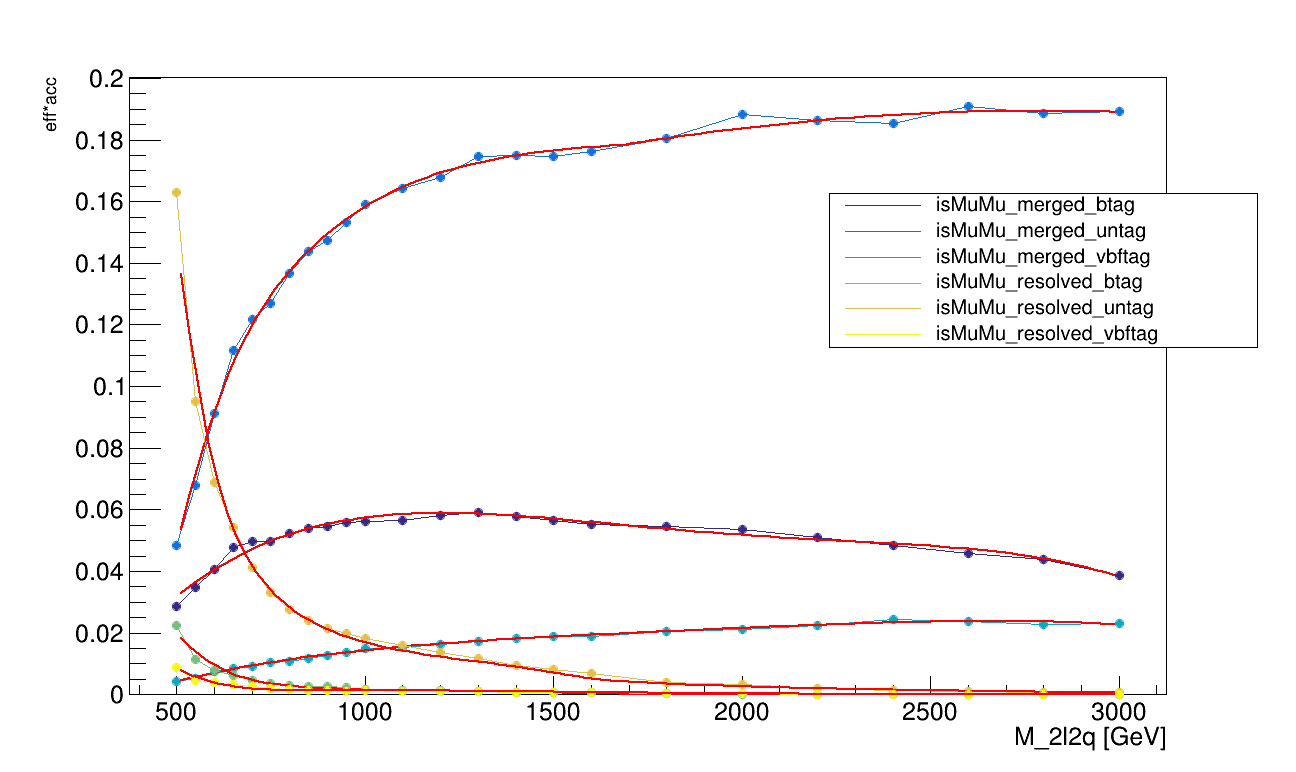
\includegraphics[width=0.45\textwidth]{figures/HighMassSearches/Efficiency/eff_ggh_isMuMu.png}\\
 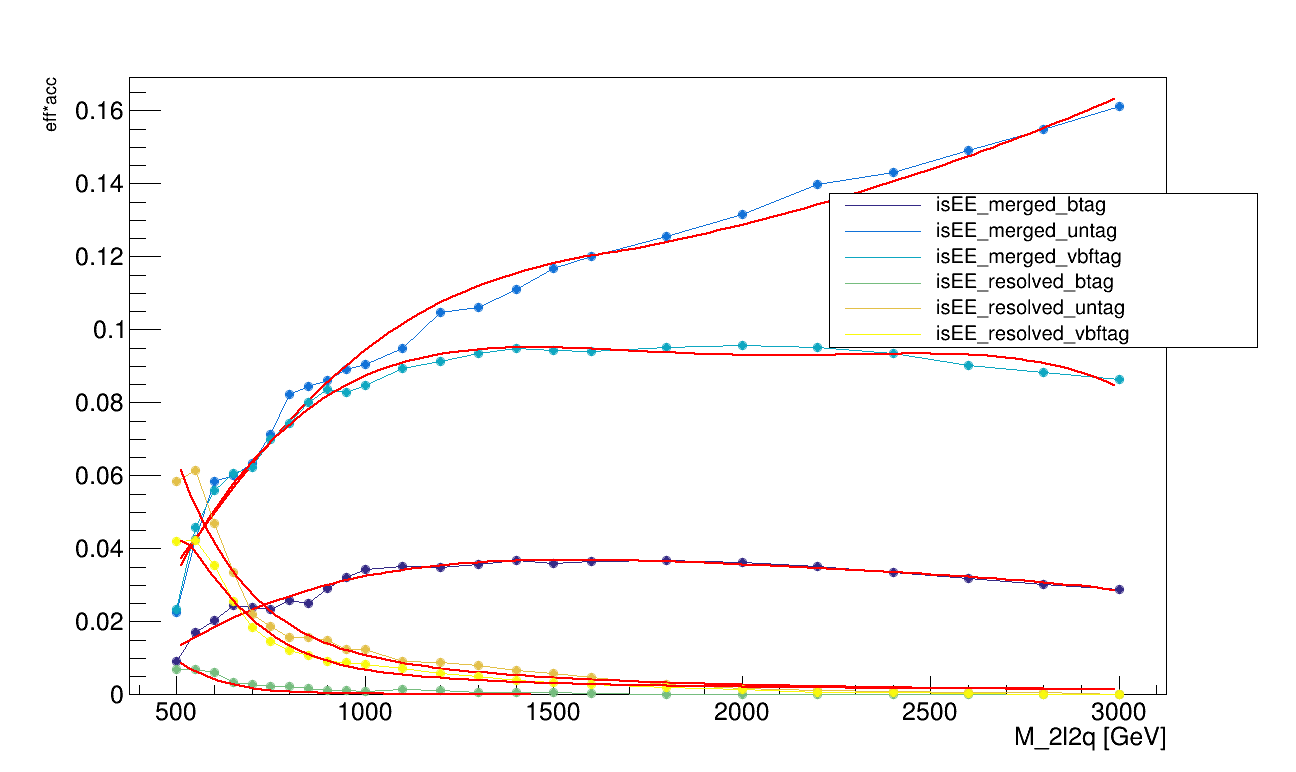
\includegraphics[width=0.45\textwidth]{figures/HighMassSearches/Efficiency/eff_vbf_isEE.png}
 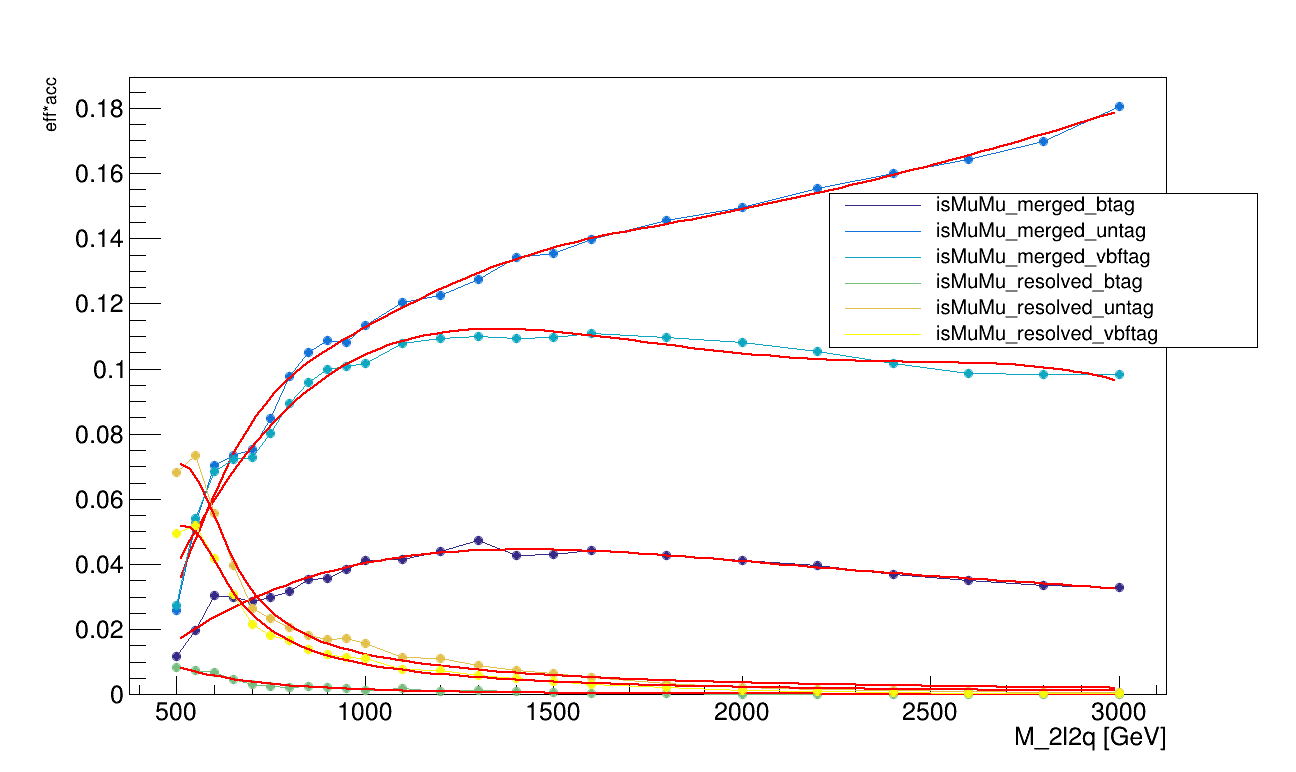
\includegraphics[width=0.45\textwidth]{figures/HighMassSearches/Efficiency/eff_vbf_isMuMu.png}\\
     % \missingfigure{efficiency plot}
 \caption{
     The product of efficiency and acceptance for signal events to pass selection as a function of the generated mass $m_{\cPZ\cPZ}^{\mathrm{Gen}}$, for \ggF (top) and VBF (bottom) production modes.
     The left panels represent the electron channels, while the right panels correspond to the muon channels.
 \label{fig:eff}
 }
 \end{figure}

 The 2D signal distributions in the final states are built with the conditional template ${\cal T}(\Dbkg|m_{\cPZ\cPZ})$,
 which describes the $\Dbkg$ discriminant distribution from Eq.~(\ref{eq:Dbkgmela}) or~(\ref{eq:Zjjmela})
 for each value of $m_{\cPZ\cPZ}$:

 \begin{eqnarray}
 {\cal P}^{i, k}_{vv}(m_{\cPZ\cPZ},\Dbkg)={\cal M}^{\mathrm{reco}}_{vv}(m_{\cPZ\cPZ})  {\cal T}(\Dbkg|m_{\cPZ\cPZ}).
 \label{eq:signalpdf2D}
 \end{eqnarray}

 The template ${\cal T}(\Dbkg|m_{\cPZ\cPZ})$ parameterization includes all detector effects
 affecting the $\Dbkg$ distribution. A closure of the full model described by Eq.~(\ref{eq:signalpdf2D})
 is achieved by comparing the model to the simulation for a number of
 signal parameters.


 \subsection{Background model}
 \label{sec:Background}
 Common backgrounds among the three final states include the $\Pg\Pg(\PV\PV)\to \cPZ\cPZ$ process, $\cPZ\cPZ$ produced via $\qqbar$ annihilation, as well as the
 $\PW\cPZ$ production process.
 The \ggF and EW production of the $\Pg\Pg(\PV\PV)\to \cPZ\cPZ$ background are treated together with the $\PX$ boson
 signal and background, including interference between the corresponding amplitudes, as discussed in detail in Section~\ref{sec:Signalmodel}. Higher order corrections are applied to these processes as discussed in Section~\ref{sec:MC}.

 The production of $\cPZ\cPZ$ via $\Pq\Paq$ annihilation is estimated using simulation. The fully differential cross section for the \qqZZ\ process is computed at NNLO~\cite{Grazzini2015407},
 and the NNLO/NLO K factor as a function of $m_{\cPZ\cPZ}$ is applied to the {\sc POWHEG} sample.
 This K factor varies from 1.0 to 1.2 and is 1.1 at $m_{\cPZ\cPZ}=125\GeV$.
 Additional NLO EW corrections, which depend on the flavor of the initial state quarks and on kinematic properties, are also applied in the region $m_{\cPZ \cPZ}>2m_{\cPZ}$, where the corrections are computed~\cite{Gieseke:2014gka,Manohar:2016nzj,Baglio:2013toa}. The $\PW\cPZ$ production is estimated using simulation, where photon induced EW corrections are applied~\cite{Frixione:2015zaa,Frixione:2014qaa}.

 The analysis specific background processes, or the ones whose contribution is derived from control samples in data, are discussed in the following sections.

 The majority of the background ($>$90\%) is composed of events from
 $\cPZ + \text{jets}$ production,
 where jets associated to the Drell--Yan production are misidentified as
 coming from a hadronic \cPZ\ decay. Subdominant backgrounds comprise
 events from \ttbar{} production and from diboson EW production.

%  The $\ttbar$ background is an important source of contamination
%  in the \cPqb\ tagged category. It is estimated from data using $\EMJWG$
%  events passing the same selection as for the signal.
%  This method accounts for other small backgrounds
%  (such as $\PW\PW + \text{jets}$, $\cPZ\to\TT + \text{jets}$, and
%  single top quark production) where the lepton flavor symmetry can be used as well.
%  Because of the limited number of events in the $\EMJWG$ control region, the \mZZ{} shapes are
%  taken from \ttbar\ simulation, and the statistical uncertainty in the control region is considered as the uncertainty in the background estimation.

 In the $\cPZ +$ jets background, the misidentified hadronic \cPZ\ comes either from
 the combinatoric background of $\cPZ + 2$ jets events where the dijet system happens to have an invariant mass
 in the range compatible with that of the $\cPZ$ boson (resolved category)
 or from an unusual parton shower and hadronization development for a single jet, leading to a configuration similar to that of the boosted $\PZ\to\qqbar$  decay (merged category). In both cases, and in each analysis category, a sideband region with a misidentified hadronic \cPZ\ mass close to that
 of the signal region can be used to estimate the contribution of this background. To address the correlation
 between the hadronic \cPZ\ mass and \mZZ{} in these configurations, a correction factor is estimated from simulation.

 \par The alpha transfer factor $\alpha(\mZZ{})$, defined as
 \begin{equation}
     \alpha(\mZZ{}) = \frac{N_\textrm{SIG}^\textrm{MC}(\mZZ{})}
     {N_\textrm{SB}^\textrm{MC}(\mZZ{})},
 \end{equation}

 is calculated as the ratio of the \mZZ{} distributions in the signal and sideband regions for $\cPZ + \text{jets}$ simulated events.
 The alpha function is multiplied by the sideband \mZZ{} distribution to derive the $\cPZ + \text{jets}$ contribution in the signal region.
 The $\cPZ + \text{jets}$ distribution from the sideband is obtained by subtracting the subdominant backgrounds from MC prediction. Both the shape and the yield for the $\cPZ + \text{jets}$ background are estimated using this method.

 While a binned evaluation of the product of the alpha factor and the sideband yields would
 be a complete estimate of the background, low event yields from data or simulation in specific
 bins or event categories could induce large statistical fluctuations
 in the bins with smaller event yields, occurring at large values of \mZZ.
 We define a ``transition'' mass value \mZZtilde. For $\mZZ < \mZZtilde$, the
 binned evaluation is used as mentioned above. For $\mZZ > \mZZtilde$,
 in order to smooth the background estimation, the $\cPZ + \text{jets}$ shape is then fit using a sum of two exponential functions (a single exponential function) for the resolved jet untagged category (the remaining categories). A binned estimation
 for $\mZZ > \mZZtilde$ is then obtained by integrating the smoothed
 estimation in the corresponding intervals. The statistical uncertainty derived from the fit is propagated to the final result using the full covariance matrix.

% \include{chapters/differentialFiducialXS_H4l}
% \include{chapters/EFTStudies}
\include{chapters/aTGC}
% \include{chapters/massMeasurement}
% \include{chapters/VH}
% \include{chapters/egamma}
% \include{chapters/hgcal}

% Results and Conclusion
% \include{chapters/results}
% \include{chapters/conclusion}

% Bibliography
\bibliographystyle{unsrt} % or preferred style
\bibliography{references,references_object_selections,references_highMassSearches} % references.bib

% Appendices
\appendix
\include{appendix/appendix}
\chapter{Modified Photon Identification}
\label{appendix:ModifiedPhotonID}

Photon identification is a crucial aspect of this analysis.
To address specific challenges in the boosted regime, where two photons are in close proximity,
we implemented a modified version of the official photon ID~\cite{Sirunyan:2018ouh}.

The original photon ID employs a boosted decision tree (BDT) classifier to effectively distinguish prompt photons from
photon candidates arising from misidentified jet fragments.
The BDT is trained on simulated $\gamma + \text{jet}$ events, where prompt photons serve as the signal and
non-prompt photons as the background.
The following variables are used as inputs to the BDT:

\begin{enumerate}
    \item \textbf{Shower shape observables}, corrected to address discrepancies between data and simulation.
    \item \textbf{Isolation variables:}
    \begin{enumerate}
        \item Photon isolation ($I_\text{ph}$) and charged hadron isolation ($I_\text{ch}$).
        \item Two types of charged hadron isolation are computed:
        \begin{enumerate}
            \item Using hadrons associated with the chosen primary vertex.
            \item Using hadrons from the vertex contributing the largest isolation sum, effectively rejecting photon candidates originating from jets associated with other vertices.
        \end{enumerate}
    \end{enumerate}
    \item \textbf{Photon pseudorapidity} ($\eta$) and energy, which are correlated with the shower topology and isolation variables.
    \item \textbf{Median energy density per unit area} ($\rho$), to minimize the effects of pileup.
\end{enumerate}

In the boosted regime, where two photons are close to each other, the energy deposition of one photon can significantly impact the photon
isolation calculation of the other.
To mitigate this effect, we modified the evaluation of the photon ID BDT by setting the "PF photon isolation" variable
 to a constant value of 0.
 This adjustment ensures that the energy contribution from a nearby photon does not influence the photon ID score.

The remaining input variables were kept unchanged, and the official EGamma photon ID model was used to compute the modified photon ID scores.
This modification enhances the performance of photon identification in the boosted regime, improving the separation between signal and background.
The effect of this modification is illustrated in Figure~\ref{fig:BeforeAfterScorePhotonIDModifications}.
\begin{figure}[!htbp]
    \centering
    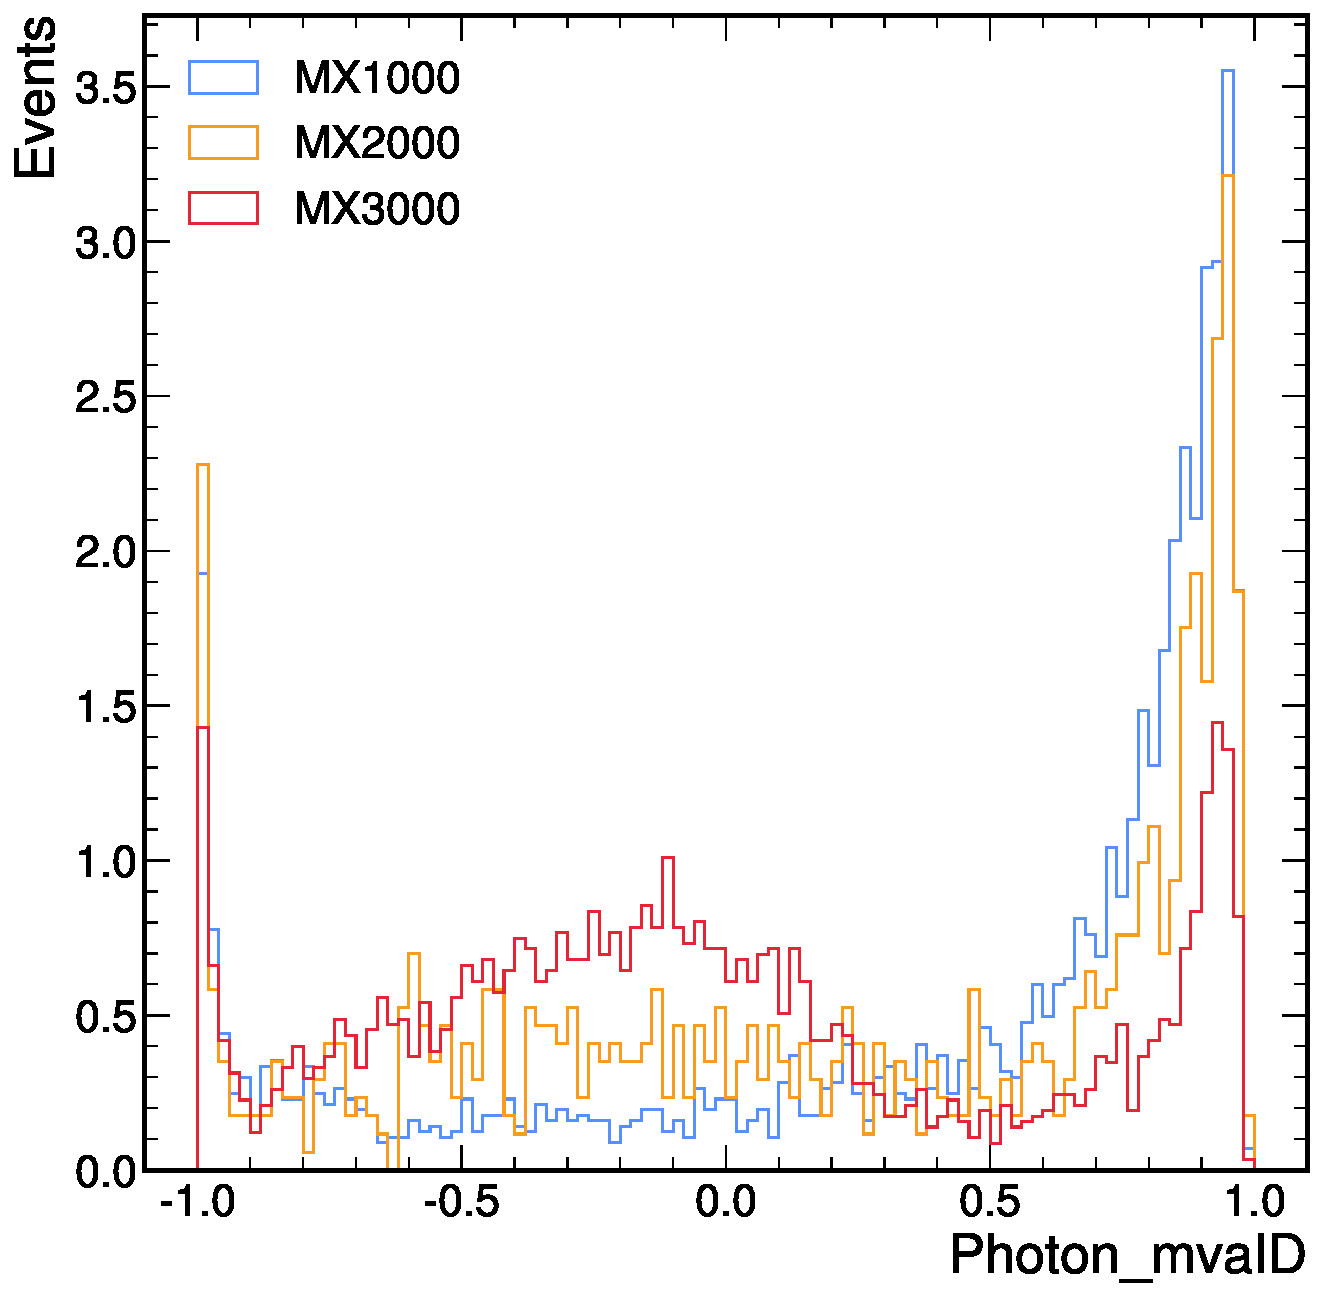
\includegraphics[width=0.45\textwidth]{figures/appendix/ModifiedPhotonID/EGamma_PhotonmvaID_3Xmass.pdf}%
    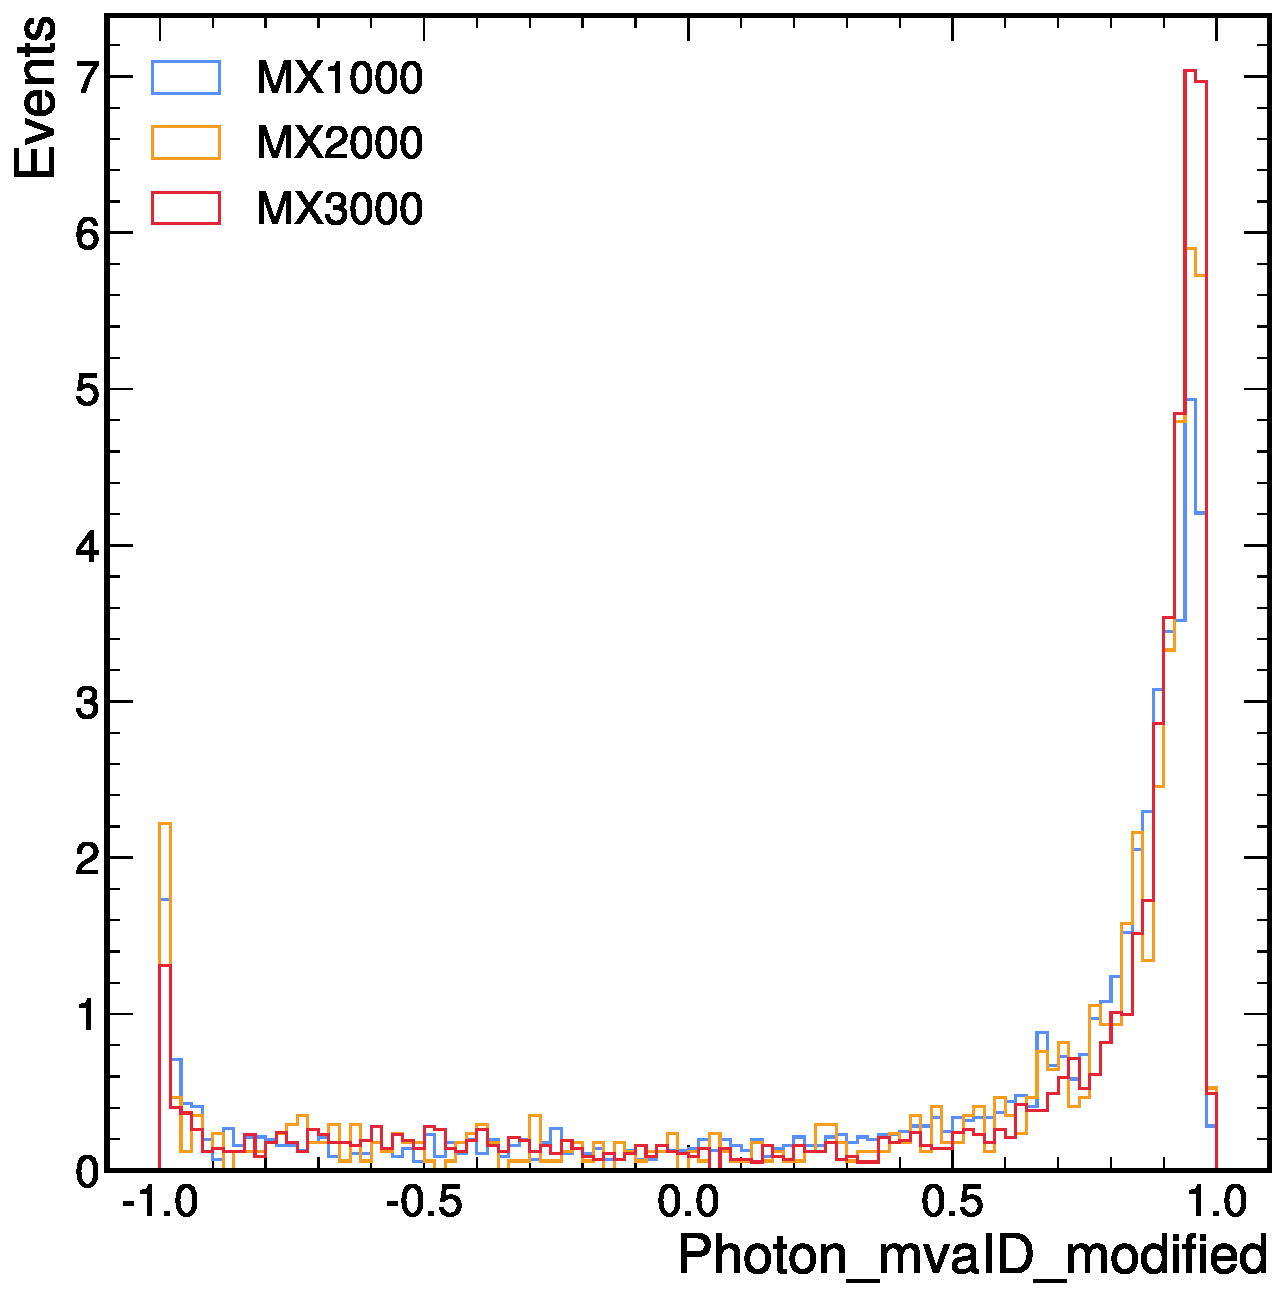
\includegraphics[width=0.45\textwidth]{figures/appendix/ModifiedPhotonID/PhotonmvaID_modified_3Xmass.pdf}
    \caption{Comparison of the photon ID score distributions before and after the modifications.}
    \label{fig:BeforeAfterScorePhotonIDModifications}
\end{figure}

For the analysis, we adopted a threshold of $\text{Modified Photon ID} > -0.7$ as a preselection criterion.
This threshold strikes a balance between retaining sufficient signal statistics for further extraction and suppressing background contributions effectively.

The modified photon ID was validated using the same data-driven techniques as the original ID, including $Z \to e^+e^-$ and $Z \to \mu^+\mu^-\gamma$ events.
These validations demonstrated that the modified photon ID retains high efficiency and reliability across various photon categories,
especially in the boosted regime.


\end{document}
